\documentclass[a4paper,10pt]{article}

\usepackage{subfig}
% Paquetes
% \usepackage{fontspec}
\usepackage{titlesec}
\usepackage{titling}
\usepackage{setspace}
\usepackage[hidelinks]{hyperref}
\usepackage{graphicx}
\usepackage{caption}
\usepackage{subcaption}
\usepackage{float}
\usepackage{xcolor}
\usepackage[affil-it]{authblk}
% \usepackage{biblatex}
% \addbibresource{Mendeley.bib}

% Para tablas
\usepackage{booktabs}
\usepackage{longtable}
\usepackage{rotating}

% Idioma
\usepackage[spanish,es-tabla]{babel}
\usepackage[utf8]{inputenc}
% \setlength{\parskip}{1em}
% Configuraciones
% \setmainfont{Times New Roman}
\hypersetup{
    colorlinks,
    linkcolor={red!50!black},
    citecolor={blue!50!black},
    urlcolor={blue!80!black}
}

\usepackage{mathrsfs}
\usepackage{amsmath,amssymb}
\usepackage{bm}
% \setlength{\parskip}{1em}
\begin{document}
\begin{titlepage}
\centering
\begin{figure}[t]
	\centering
	
\includegraphics[scale=0.15]{utn.jpg}
    \vspace{0.5cm}
\end{figure}%
	{\LARGE Proyecto Final\par}
    {\LARGE 2018\par}
	\vspace{1cm}
	{\huge\bfseries Robots con detección de entorno\par}
	\vspace{1cm}
    {\LARGE Tesina\par}
    \vspace{1cm}
	{\Large\itshape Domínguez, Francisco\par}
	\vfill
\end{titlepage}


\tableofcontents

\newpage
\listoffigures
\newpage
\listoftables

\newpage
\section*{Objeto del Documento}
\label{sec:0_objeto}
El objeto del presente es hacer un análisis exhaustivo del estado de las plataformas de Hardware presentes en el mercado actual, de manera de diseñar a partir de dicho análisis una plataforma versátil para el usuario que permita extender el rango de aplicaciones de las plataformas ya existentes, permitiendo así, por ejemplo, el montaje de sensores adicionales a la placa. En base a dicho diseño, se implementa una solución al problema de la localización y mapeo simultáneos (SLAM).

\newpage
\section*{Abstract}
\label{sec:1_abstract}

En los últimos años, los robots han recibido una mayor atención de la comunidad de investigación, en especial debido a la aparición de los vehículos aéreos no tripulados.

El presente trabajo describe el desarrollo de una plataforma de control de robots. Dicha plataforma cuenta con la posibilidad de expandir sus funcionalidades gracias al estándar de hardware PC/104 presente en la industria, logrando así poder desarrollar a partir de la misma tanto vehículos aéreos no tripulados (UAV) como robots terrestres, entre otros. En base a la misma, se desarrollará un robot capaz de estimar tanto su posición como el contorno del mapa en el cual se encuentra.


\newpage
\section{Introducción}
\label{sec:2_marcoteorico}
Si bien el uso de robots tiene sus orígenes principalmente en fábricas para el ensamblaje de automóviles, en los últimos años la electrónica moderna ha permitido introducirlos en otras áreas, ya sea desde electrodomésticos y juguetes de la vida cotidiana, hasta viajes espaciales con el fin de explorar planetas desconocidos. Esta expansión es debido a que los mismos permiten reducir la interacción humana no solo en tareas que presentan un riesgo a la integridad de la persona, sino también en aquellas que tienen cierto grado de repetitividad.

Yendo a un caso más concreto, en el último tiempo muchas personas han adquirido los llamados robots aspiradoras, como el que se observa en la Figura \ref{fig:vaccumrobot}.a, los cuales consiguen limpiar la superficie de las casas en un tiempo medianamente razonable, aunque este tiempo no suele ser una preocupación ya que al ser el mismo completamente autónomo, uno puede seguir con sus actividades cotidianas. 

No obstante, si se analiza el recorrido que realizan la mayoría de estos robots, se puede apreciar que el mismo suele ser completamente aleatorio, y por ende se tendería a creer que no podrá pasar por toda la superficie y limpiarla completamente. La realidad es que, como están mucho tiempo circulando, logran pasar por todos los rincones de la superficie, pero esto genera que circulen más veces por unos lugares que por otros, tal como se observa en la Figura \ref{fig:vaccumrobot}.b, haciendo ineficiente el trabajo.

\begin{figure}[!ht]
    \centering
    \subfloat[Robot aspiradora comercial]{{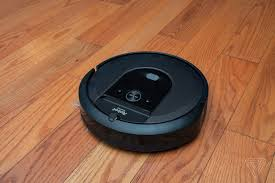
\includegraphics[width=0.47\textwidth]{Img/Roomba}}}%
    \qquad
    \subfloat[Ejemplo del recorrido de un robot aspiradora comercial]{{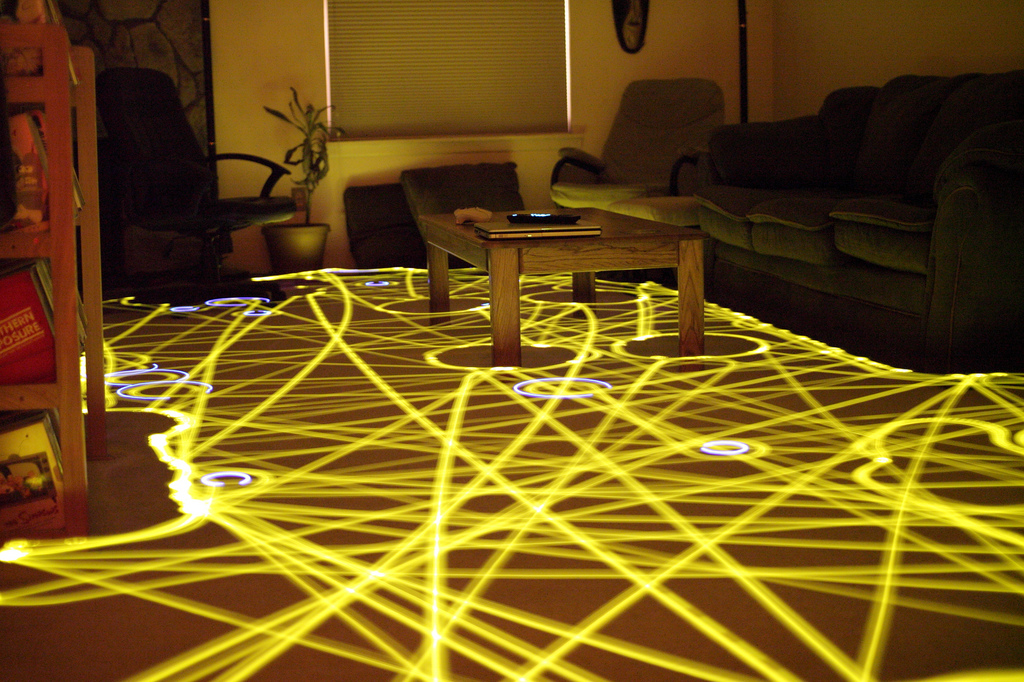
\includegraphics[width=0.47\textwidth]{Img/VaccumRobot.png}}}%
    \caption{El robot aspiradora}
    \label{fig:vaccumrobot}
\end{figure}

\ifimagenes
Si lo que se pretende es optimizar el recorrido del robot, la
\else
A pesar de que se busque reducir la interacción humana bajo estas circunstancias, no todos los robots hoy en día son autónomos, principalmente debido a la falta de robustez del algoritmo de control involucrado en el proceso. Tomando por caso el ejemplo anterior, si bien el robot aspiradora es autónomo, su eficiencia respecto a la forma óptima de realizar la tarea no es una garantía en todos los casos.

Es útil distinguir entre robots que están inmóviles, como un brazo robótico en una fábrica, y robots que son móviles, como un auto sin conductor. En este trabajo se hará hincapié en los robots móviles. Usamos este término para describir un robot impulsado por sus propios medios que puede moverse cinemáticamente entre ubicaciones en su entorno. A su vez, cuando se habla de la posición y orientación combinadas del robot, esto se define como su \textit{pose}.

Los robots móviles pueden referirse a robots que se mueven sobre el suelo, bajo el agua, a través del aire y en entornos de microgravedad, tales como los que pueden observarse en la Figura \ref{fig:mobilerobots}. Si bien este trabajo busca aplicar en parte a cualquiera de estos entornos, el enfoque del mismo se refiere principalmente a los robots móviles que permanecen en contacto con el suelo. Cada uno de ellos presentan su propia terminología para definirlos y diferenciarlos del resto, por ejemplo, el término vehículos terrestres no tripulados o UGV (del inglés \textit{unmanned ground vehicles}) a menudo se usa más específicamente para describir robots móviles terrestres, mientras que el término vehículos aéreos no tripulados o UAV (del inglés \textit{unmanned aerieal vehicles}) refieren principalmente a los drones.

Los robots móviles se mueven a través de entornos grandes y potencialmente dinámicos, lo que hace que la percepción sea mucho más difícil que los robots industriales con entornos de trabajo limitados y parámetros operativos rígidos. Por lo tanto, los robots móviles requieren sensores adicionales, una mejor percepción y mayores grados de autonomía para operar en entornos del mundo real que cambian con frecuencia.


\begin{figure}%
    \centering
    \subfloat[Wheeled robot]{{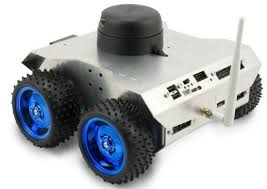
\includegraphics[width=0.25\linewidth]{Img/WheeledRobot.jpeg}}}%
    \qquad
    \subfloat[Legged robot]{{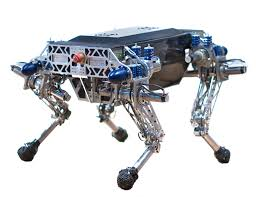
\includegraphics[width=0.25\linewidth]{Img/LeggedRobot.jpeg}}}%
    \qquad
    \subfloat[Tracked robot]{{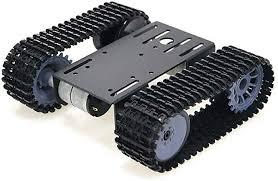
\includegraphics[width=0.25\linewidth]{Img/TrackedRobot.jpeg}}}%
    \qquad
    \subfloat[Drone]{{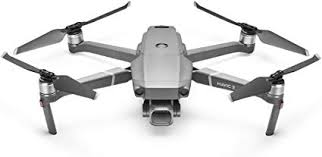
\includegraphics[width=0.3\linewidth]{Img/Drone.jpeg}}}%
    \qquad
    \subfloat[Water-based robot]{{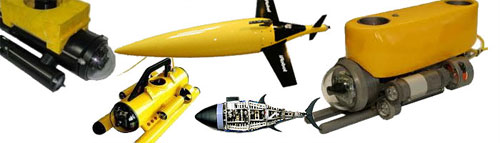
\includegraphics[width=0.5\linewidth]{Img/WaterBasedRobot.jpg}}}%
    \caption{Tipos de robot móviles}
    \label{fig:mobilerobots}
\end{figure}

Dentro de lo que respecta a robótica móvil, uno de sus desafíos actuales es lograr la completa autonomía del vehículo. Una gran parte de las empresas de la industria automotriz han dedicado mucho tiempo y dinero para lograr el objetivo. La investigación ha avanzado hasta el punto de que en la actualidad hay autos semi-autónomos disponibles en el mercado, y se cree ampliamente que en el futuro cercano casi todos los vehículos serán completamente autónomos. Para lograr esto, obviamente hay una necesidad de sensores y funciones avanzadas. Uno de los principales problemas es el hecho de que el vehículo debe ser consciente de su posición actual dentro de un entorno desconocido. Este proceso de determinar no solo su posición, sino también el mapa que lo rodea se conoce como la \textit{localización y mapeo simultáneos}, comúnmente abreviado como \textit{SLAM} (del inglés, \textit{simultaneous localization and mapping}).

El SLAM es un problema difícil de solucionar, así como lo fue para los humanos en el pasado. Tiempo atrás, los marineros usaban los llamados registros de fichas para estimar su velocidad y extrapolaban esta velocidad con el tiempo para calcular su pose. Este proceso de navegación por estima (en inglés, \textit{dead reckoning}) conduce inevitablemente a errores graves de posicionamiento con el tiempo y, por lo tanto, siempre se ha respaldado mediante el uso de puntos de referencia (o \textit{landmarks}) para la navegación. Quedándonos en este caso particular, con el uso de las estrellas los marineros lograban saber donde estaba el Norte, permitiendo corregir su dirección. Sin embargo, no siempre se podía observar este patrón por días debido al cielo nublado, entonces tenían que confiar solamente en su navegación por estima, haciendo que la incertidumbre crezca día tras día. Para el caso de los robots, cuando el mismo recorre un mapa completamente desconocido, acumulará error debido a las predicciones que debe tomar respecto a su pose y entorno en el que está, hasta el momento en que entra a un área con puntos de referencia conocidos, pudiendo así corregir su estimación de posición.

Volviendo al ejemplo del robot de limpieza, si el mismo conociera el mapa en el que se encuentra, podría entonces trazar la ruta mas óptima para realizar la limpieza del lugar. Como no todos los ambientes son iguales y cada uno tiene, por ejemplo, muebles ubicados en distintos lugares, dicho robot podría hacer primero un reconocimiento del lugar previo a la limpieza para tener una noción de todo el espacio, o bien obtener el mapa y la ubicación en la que se encuentra en base al movimiento que realiza, pasando por los lugares que le faltaron aspirar. Para cualquiera de las dos opciones, por lo tanto, necesitará tanto tomar los datos del lugar como controlar al vehículo para que vaya circulando por el ambiente.

La
\fi
estimación de la pose, entonces, es una parte no separable de aplicaciones como el control del vehículo y el mapeo. Varios sensores se utilizan comúnmente para estimar la pose de un robot. Las unidades de medición inercial (IMU), la cámara, la odometría de las ruedas\footnote{Se mide la rotación de las ruedas para estimar cambios de la posición del vehículo a lo largo del tiempo} para el caso de ciertos robots móviles y el LiDAR se encuentran entre los sensores más populares para la localización en interiores \cite{delrosario2016}, mientras que para exteriores suele sumarse el GPS a estos sensores, corrigiendo al mismo mediante acción de la IMU \cite{caron2006}.


\ifimagenes
\else
En la localización al aire libre, la señal del sistema de posicionamiento global (GPS) suele estar disponible y, dado que la posición se puede obtener con precisión mediante GPS, es la opción común para la fusión con los datos obtenidos de la IMU \cite{engel2014}. Sin embargo, en un entorno denegado por GPS, como dentro de un edificio, se deben usar otros sensores para corregir las estimaciones de la IMU. Un enfoque común para abordar este problema son la fusión IMU-cámara \cite{mirzaei2008}, \cite{hesch2009}, \cite{chambers2014}, \cite{hesch2013}, así como también el uso de LiDAR \cite{lee2016}.

Un algoritmo SLAM robusto es esencial para que cualquier robot móvil navegue de manera segura a través de un entorno no estructurado. El algoritmo SLAM con frecuencia define un marco de coordenadas global para que el robot opere; uno que generalmente es utilizado por todas las funcionalidades de alto nivel, como navegación, planificación de rutas, exploración, identificación de objetos, seguimiento de objetos y manipulación de los mismos. Estas dependencias hacen que el algoritmo SLAM sea una parte central de cualquier arquitectura de robot móvil, y las fallas irrecuperables son altamente indeseables. Es probable que cualquier robot desorientado por una falla de SLAM no pueda realizar su tarea, o peor, puede poner en peligro a los humanos, a sí mismo o al medio ambiente.

%Si bien se han demostrado varios algoritmos SLAM en laboratorios, es más difícil producir soluciones robustas en entornos no estructurados del mundo real. El deslizamiento de las ruedas, por ejemplo, puede producir mediciones de odometría ruidosas, mientras que los sensores del sistema de posicionamiento global (GPS) a menudo producen una localización global con saltos muy pronunciados para la misma posición. El SLAM robusto del mundo real se vuelve aún más difícil cuando estos errores de detección aleatorios y sistemáticos ocurren en entornos que tienen geometrías redundantes u objetos en movimiento. Por ejemplo, en el caso de los LIDAR bidimensionales, los algoritmos empleados con los mismos suelen presuponer que el robot se encuentra terrestre se encuentra sobre una superficie plana, tal como puede ser el cuarto de un hogar. Si la superficie presenta irregularidades muy marcadas, la tarea de mapeo en dos dimensiones del mismo aumentaría su complejidad, ya que no podría encontrar las relaciones entre los datos anteriores con los actuales (no coincidirían) por si solo, y dependería de sensores adicionales, como una IMU.

%Para poder realizar las tareas en tiempo real, es necesario contar con una capacidad de cómputo suficiente para no sólo adquirir todos los datos de los sensores, sino también procesarlos para conseguir el mapa junto a la pose en cada momento. En el presente trabajo, se desarrolla una plataforma de Hardware capaz de realizar dicha actividad, a su vez de describir dos algoritmos de SLAM, uno basado en la combinación de un LIDAR 2D junto a una IMU, y el otro basado en una cámara RGB-D, obteniendo entonces un SLAM tridimensional.
\fi



En particular, para el caso de la localización y mapeo tridimensional (SLAM 3D), los LIDAR 3D han adquirido bastante popularidad en el último tiempo con la llegada de los vehículos autónomos, aunque son muy costosos. Si se pretende entonces una opción más económica, las cámaras estéreo y RGB-D (\textit{D: Depth - profundidad}) son de las más utilizadas para esto, a su vez de poder obtener datos de color de las mismas. Los sensores RGB-D como la \textit{Microsoft Kinect} proporcionan directamente mapas de profundidad densos e imágenes en color. En general, los enfoques SLAM que operan en imágenes RGB-D son estructuralmente diferentes de los sistemas estéreo, ya que la entrada es RGB-D de profundidad en lugar de dos imágenes de color. A pesar de esto, pueden obtenerse nubes de puntos de profundidad a partir de ambos sensores con el procesamiento
\ifimagenes
\ifimagenespaper
adecuado, como los presentados por la librería OpenCV \cite{kaehler2017}.
\else
adecuado, lo cual se desarrolla en el apéndice.
\fi
\else
adecuado, como los presentados por la librería OpenCV \cite{kaehler2017}.
\fi

Una vez obtenidas las nubes de puntos de profundidad, una de las formas de calcular la posición y orientación del robot (conocido como la \textit{pose} del robot) a lo largo del tiempo es mediante la comparación entre dos nubes de puntos contiguas (una con los datos recientes y otra con los datos de la nube de puntos anterior), buscando en definitiva la transformación necesaria para que la nube de puntos actual pueda alinearse (o sea, que coincida lo mejor posible) con la nube de puntos anterior. Este proceso se lo conoce como el \textit{registro de la nube de puntos}, y suele llevar una serie de pasos, lo cual se desarrollará más adelante. Para poder facilitar el uso de nubes de puntos, existen librerías específicas para trabajar con dicha información, siendo algunas de ellas la \textit{Point Cloud Library} y \textit{Open3D}, las cuales implementan no sólo distintos algoritmos, sino también estructuras para facilitar el manejo de las nubes de puntos.

Si bien hay muchos robots móviles hoy en día en el mercado, gran parte de ellos son costosos, y sobre todo los que se encuentran equipados para realizar SLAM 3D. Para poder evaluar los algoritmos necesarios sin tener que ponerse en gasto, existen entornos de simulación pensados, entre otras cosas, para robots, consiguiendo resultados comparables con los reales. Unos de los más conocidos en el ámbito son \textit{V-REP} y \textit{Gazebo}, siendo este último el elegido para realizar el trabajo.

\subsection{Contribuciones}
En el presente trabajo, 
\ifimagenes
se desarrolla un algoritmo de registro de nube de puntos en base a los datos obtenidos de una cámara RGB-D en movimiento dentro de un ambiente estático, bajo el entorno de simulación Gazebo. En base a la transformación obtenida en cada iteración, se aplica la misma a la nube de puntos entrante, para luego sumarla al mapa 3D generado.

Como el trabajo presentado forma parte de una tesis de grado en desarrollo sobre SLAM 2D y 3D, se pretende que el mismo pueda fusionarse con los datos provenientes de otros sensores, en particular la IMU y el LIDAR 2D, para obtener una mejor estimación de la posición y, por consiguiente, obtener un mapa más exacto.

\else
se presenta una plataforma de Hardware capaz de realizar las tareas de SLAM que incluyen una gran cantidad de sensores, a su vez de contar la misma con un factor de forma de Hardware para que la misma pueda expandir sus funcionalidades en base a lo que requiera el usuario.

Luego, e describen dos algoritmos de SLAM, uno basado en la combinación de un LIDAR 2D junto a una IMU, y el otro basado en una cámara RGB-D, obteniendo entonces un SLAM tridimensional, ambos considerando un entorno estático. Debido a la falta de sensores capaces de brindar la información reuqerida, se realizaron las pruebas del mismo bajo el entorno de simulación Gazebo, con el fin de poder luego llevarlas a un escenario real cuando se tenga el robot completo.
\fi

A su vez, se provee de un código compatible con \textit{ROS}, un framework pensado para utilizar en robótica, permitiendo portabilidad y versatilidad a la hora de proporcionar los datos de los sensores, ya que el mismo utiliza un sistema de mensajes que permite vincular a dos procesos sin importar el método de adquisición o procesamiento de los datos, mientras los mismos respeten el tipo de mensaje en sí.

\subsection{Estructura del documento}
El presente documento se compone de las siguientes secciones
\ifimagenespaper
\else
y apéndices
\fi
\begin{itemize}
    \item \textbf{Introducción}: esta sección hace una breve introducción al SLAM, presentando los distintos sensores utilizados normalmente, a su vez de dar una primera aproximación al registro de nubes de puntos con los sensores RGB-D para realizar dicha tarea. A su vez, se mencionan las contribuciones realizadas.
    \ifimagenespaper
    \item \textbf{Marco teórico}:
    \else
    \item \textbf{Herramientas para el desarrollo de robots}: En esta sección se da una introducción al framework \textit{ROS}, en particular a su estructura y su modo de vinculación entre los distintos paquetes. Finalmente, se da una breve descripción de Gazebo.
        \ifimagenes
    \item \textbf{Marco teórico}:
        \else
    \item \textbf{Geometría tridimensional y marcos de referencia}: en esta sección se desarrollan los conceptos de la geometría tridimensional necesarias para abordar los temas del trabajo realizado, a su vez de mencionar distintos marcos de referencia usualmente utilizados.
    \item \textbf{Análisis de regresión}: en esta sección se desarrolla el denominado análisis de regresión, abarcando tanto la regresión lineal como la no lineal.
    \item \textbf{Estimación de estado}: siguiendo con el análisis de regresión, en esta sección se desarrollan distintos algoritmos de estimación de estado, siendo uno de los mas conocidos el filtro de Kalman.
    \item \textbf{Sensores}: en esta sección se mencionan distintos sensores utilizados comúnmente en lo que refiere al SLAM, a su vez de presentar distintos métodos de calibración de algunos de ellos y características importantes.
    \item \textbf{Simultaneous Localization And Mapping}: en esta sección se profundiza en lo que refiere al SLAM, mencionando no sólo distintos algoritmos que existen, sino también mencionando características importantes de la técnica en si.
    \item \textbf{Reconstrucción del entorno}:
        \fi
    \fi 
    en esta sección se describe tanto el flujo de trabajo del registro de nubes de puntos asi como también los distintos algoritmos utilizados comúnmente a la hora de realizarlo, asociando a los mismos con su implementación en la librería PCL. A su vez, se comenta como conseguir las nubes de puntos en base a los sensores utilizados comúnmente en este tipo de
    \ifimagenes
    aplicaciones, además de una calibración de los mismos.
    \item \textbf{Experimentos}: En base a la sección anterior, en esta se describe el flujo del algoritmo realizado, además de presentar los resultados obtenidos en base a la simulación realizada
    \else
    aplicaciones.
    \item \textbf{Plataformas disponibles}: en base a los sensores y datos necesarios, en esta sección se realiza un relevamiento de las distintas plataformas disponibles en el mercado, comparando cada una de ellas.
    \item \textbf{Resolución}: en esta sección se mencionan los métodos utilizados para lograr el objetivo del trabajo, basándose en las secciones anteriores. A su vez, se muestran los resultados obtenidos.
    \fi
    \item \textbf{Conclusiones}: En esta sección se desarrolla la finalidad conseguida del trabajo, evaluando distintos puntos de interés.
    \ifimagenes
    \item \textbf{Trabajos futuros}: en esta sección se mencionan distintos aspectos para lo que sigue luego de este trabajo.
    \else
    \item \textbf{Apéndices}: en esta sección se incluye información útil, como el esquemático de la placa realizada.
        \ifimagenespaper
        \else
    \item \textbf{Anexo}: Finalmente, se incluye un anexo con información útil a la hora de querer llevar a cabo una implementación con sensores físicos, utilizando los datos proporcionados por los mismos.
        \fi
    \fi
\end{itemize}

\subsection{Resumen}
En esta Sección se dio una introducción respecto a los temas que va a abordar el trabajo realizado, a su vez de mencionar las contribuciones por el mismo y, finalmente, mencionar las distintas secciones que se incluyen.

\newpage
% Regression analysis o state estimation?
\section{Estimación de estado}
La estimación de estado consiste en determinar el estado no medible de un sistema dinámico a partir de las mediciones de entrada y salida de dicho sistema. Lamentablemente, las mediciones no son perfectas, lo que conduce a una inexactitud inherente en el valor de la medición. Para tener en cuenta estos errores, la estimación de estado procesa todas las mediciones disponibles y utiliza un \textit{análisis de regresión} para identificar el estado real probable del sistema.

El análisis de regresión es un análisis estadístico para predecir el valor de una variable cuantitativa continua. Basándose en un conjunto de variables independientes, se busca estimar la relación de las mismas con una variable dependiente, mediante la obtención de una curva que mejor se ajuste a los datos disponibles, sin que necesariamente pase por todos ellos. En concreto, el modelo de regresión puede representarse como
\begin{equation}
    y_i = f(\bm{x}_i; \bm{\beta}) + v_i,
    \label{eq:regressionmodel}
\end{equation}
donde la variable $y_i$ corresponde a la respuesta o medición para el caso $i$, con $i = 1, 2, ..., m$, $\bm{x}_i = (x_{i1}, x_{i2}, ..., x_{in})$ corresponde al conjunto de valores, fijos o aleatorios, utilizados para explicar o predecir el comportamiento de $y_i$, conocidos como las \textit{variables regresivas} o independientes, $\bm{\beta} = (\beta_1, \beta_2, ..., \beta_n)$ a los parámetros desconocidos\footnote{A diferencia de un estado, el que se define como una magnitud física que varía a través del tiempo, el parámetro es constante a través del tiempo.} a estimar, y $v_i$ a la componente de ruido propia para ese caso.

En base a esto, lo que se busca es estimar la función $f$ que mejor se ajuste a los datos, conocida como \textit{función de expectativa} para el modelo de regresión. Para ello, primero lo que debe hacerse es determinar la forma de dicha función. En base a la forma que adquiera la misma, se puede clasificar en \textit{regresión lineal} y \textit{regresión no lineal}.

Existen diferentes métodos dentro del análisis de regresión para poder estimar los parámetros desconocidos $\beta$, por lo que en las siguientes subsecciones se presentarán algunos de ellos, los cuales son de relevancia para el seguimiento de la tesis.

% En cambio, cuando la función que modela al sistema \textit{no puede expresarse como una combinación lineal de los parámetros desconocidos} $\bm{\beta}$, se trata entonces de una regresión no lineal, y debe realizarse un proceso iterativo para encontrar la curva que mejor se adapte al sistema.

% La información de tales relaciones se efectúa a partir de información muestral acerca de los valores tomados por $y$, $x_1$, $x_2$, $x_3$, ..., $x_n$, y trata de cuantificar la magnitud de la dependencia entre ellas.

\subsection{Regresión lineal}
En regresión lineal, la variable $y$ \textit{es una combinación lineal} de los parámetros, es decir,
\begin{align}
    y_i &= \beta_1 x_{i1} + \beta_2 x_{i2} + \beta_3 x_{i3} + ... + \beta_n x_{in} + v_i \\
      &= \bm{x}_i \bm{\beta} + v_i
\end{align}

Con el fin de hallar los parámetros desconocidos, uno de los métodos más utilizados corresponde al \textit{método de cuadrados mínimos}, el cual plantea que el valor más probable de los parámetros desconocidos será aquel que minimiza la suma de los errores cuadráticos entre lo que se observa y lo que se espera. Este método es una variante especial del problema más general, en el que dada una función $f:\mathbb{R}^n\rightarrow\mathbb{R}$ se busca un argumento de $f$ que de el mínimo valor de la llamada \textit{función de coste}
\begin{equation}
    \hat{x} = argmin_x f(x)
    \label{eq:globalminimizer}
\end{equation}
llamado tambien como el \textit{minimzador global}.

\subsubsection{Cuadrados mínimos ordinario}
Si se quiere, por ejemplo, medir el peso de una bolsa de naranjas, cuyo valor real es $x$, con el uso de una balanza de poca precisión, el valor medido $y$ puede modelarse como el valor real corrompido por ruido, $v$, linealmente mediante la ecuación
\begin{equation}
    y = x + v
    \label{eq:linearmeasmodel}
\end{equation}

Para cada una de las mediciones, se define un término escalar de ruido que es independiente de los otros términos de error ya que, para este caso, se asume que el ruido es independiente y de distribución uniforme. Ahora, si se define el error entre cada medición y el valor verdadero de la bolsa de naranjas, se obtiene el denominado \textit{criterio de error} de cada medición, esto es,
\begin{equation}
    e_i = y_i - x
\end{equation}

Con estos errores definidos, el método de cuadrados mínimos define que la mejor estimación del valor $x$ es la que minimiza el \textit{criterio de error cuadrático},
\begin{equation}
    \hat{x}_{LS} = argmin_x(e_1^2+e_2^2+e_3^2+e_4^2+e_5^2) = \mathscr{L}_{LS}(x),
    \label{eq:squarederrorcriterion}
\end{equation}
aunque a veces también llamada \textit{función de coste de error cuadrático} o \textit{función de pérdida}.

% Luego de un set de cinco mediciones realizadas por separado y en forma secuencial, se obtienen los valores que se observan en la Tabla \ref{tab:naranjasbalanza}, junto con sus modelos de medición y errores cuadráticos.

% \begin{table}[]
\centering
\begin{tabular}{c|c|c|c}
\textbf{Medición} & \textbf{Peso {[}g{]}} & \textbf{Modelo de medición} & \textbf{Error} \\ \hline
1                       & 1012                  & $y_1 = x + v_1$        & $e_1 = y_1 - x$      \\ \hline
2                       & 989                   & $y_2 = x + v_2$        & $e_2 = y_2 - x$      \\ \hline
3                       & 1008                  & $y_3 = x + v_3$        & $e_3 = y_3 - x$      \\ \hline
4                       & 1030                  & $y_4 = x + v_4$        & $e_4 = y_4 - x$      \\ \hline
5                       & 971                   & $y_5 = x + v_5$        & $e_5 = y_5 - x$           
\end{tabular}
\caption{Peso de una bolsa de naranjas para cada medición realizada}
\label{tab:naranjasbalanza}
\end{table}

Para poder minimizar la función de coste, suponiendo que fueron tomadas cinco mediciones realizadas por separado y en forma secuencial, primero hay que reescribir a la función de error en su forma matricial, siendo entonces
\begin{align}
    \bm{e} &= \bm{y} - \bm{H}\cdot x \\
    \begin{bmatrix}
        e_1\\ e_2\\ e_3\\ e_4\\ e_5
    \end{bmatrix}
    &= 
    \begin{bmatrix}
        y_1\\ y_2\\ y_3\\ y_4\\ y_5
    \end{bmatrix}
    -
    \begin{bmatrix}
        1\\ 1\\ 1\\ 1\\ 1
    \end{bmatrix}
    x
\end{align}
siendo $\bm{H}$ la \textit{matriz Jacobiana}. Dicha matriz tiene las dimensiones de $m\times n$, donde \textit{m} es el número de mediciones y \textit{n} es el número de parámetros que se desean estimar. Por ello, \textit{x} si bien en este caso es un escalar, puede ser un vector en el caso que se tengan múltiples indeterminaciones. En base a esto, se puede redefinir a la función de costo como

\begin{align}
    \mathscr{L}_{LS}(x) &= \bm{e}^T\bm{e} \\
                        &= (\bm{y} - \bm{H}x)^T(\bm{y} - \bm{H}x) \\
                        &= \bm{y}^T\bm{y} - x^T\bm{H}^T\bm{y} - \bm{y}^T\bm{H}x + x^T\bm{H}^T\bm{H}x
\end{align}

Para minimizar esta ecuación, se procede a computar la derivada parcial de la función de costo respecto a la incertidumbre $x$ para luego igualarla a cero.
\begin{align}
    \frac{\partial \mathscr{L}}{\partial x}\bigg\rvert_{x=\hat{x}} = -\bm{y}^T\bm{H} - \bm{y}^T\bm{H} + 2\hat{x}^T\bm{H}^T\bm{H} &= 0 \\
    -2\bm{y}^T\bm{H} + 2\hat{x}^T\bm{H}^T\bm{H} &= 0
\end{align}

Despejando, se llega al valor del peso de la bolsa de naranjas que minimiza el criterio de error cuadrático
\begin{equation}
    \hat{x}_{LS} = (\bm{H}^T\bm{H})^{-1}\bm{H}^T\bm{y}
\end{equation}

Esta expresión tiene solución si y solo si existe $(\bm{H}^T\bm{H})^{-1}$, o sea, si la matriz tiene inversa. Si tenemos \textit{m} mediciones y \textit{n} parámetros,
\begin{align*}
    \bm{H} &\in \Re^{m\times n} \\
    \bm{H}^T\bm{H} &\in \Re^{n\times n}
\end{align*}

Por lo tanto, para que $(\bm{H}^T\bm{H})^{-1}$ exista es necesario que se dispongan mínimamente de la misma cantidad de mediciones que variables a estimar, esto es
\begin{equation*}
    m \geq n
\end{equation*}

\subsubsection{Cuadrados mínimos ponderado}

Volviendo al ejemplo de la bolsa de naranjas, si se toman mediciones con distintas balanzas, es lógico pensar que mientras mayor sea la precisión de cada una, mayor importancia tendrá su valor indicado para determinar el peso de la bolsa. Si se considera al modelo de medición lineal con \textit{m} mediciones y \textit{n} incertidumbres,
\begin{align}
    \begin{bmatrix}
        y_1 \\ . \\ . \\ . \\ y_m
    \end{bmatrix}
    &=
    \bm{H}
    \begin{bmatrix}
        x_1 \\ . \\ . \\ . \\ x_n
    \end{bmatrix}
    +
    \begin{bmatrix}
        v_1 \\ .\\ . \\ . \\ v_m
    \end{bmatrix} \\
    \bm{y} &= \bm{H} \bm{x} + \bm{v}
\end{align}

En cuadrados mínimos ordinarios, se asume implícitamente que cada término de error, $v_i$, posee el mismo desvío estándar, $\sigma$. En cambio, si se toma que cada término de error es independiente pero con distinto desvío estándar,
\begin{equation}
    \mathbb{E}_{[v_i^2]} = \sigma_i^2 \hspace{0.5cm}(i=1,...,m)\hspace{1cm}\bm{R}=\mathbb{E}_{[\bm{v}\bm{v}^T]} = 
    \begin{bmatrix}
        \sigma_1^2  &        &     0      \\
                    & \ddots &            \\
            0       &        & \sigma_m^2
    \end{bmatrix}
\end{equation}
se puede definir a partir de esto el \textit{criterio de cuadrados mínimos ponderado} como
\begin{align}
    \mathscr{L}_{WLS}(x) &= \bm{e}^T\bm{R}^{-1}\bm{e} \\
                         &= \frac{e_1^2}{\sigma_1^2} + \frac{e_2^2}{\sigma_2^2} + ... + \frac{e_m^2}{\sigma_m^2}
\end{align}

Mientras mayor sea el ruido esperado, menor será el peso que tenga en la medición. En el caso que todos los desvíos sean iguales, \textit{no afecta el valor estimado final}, ya que pasa a ser una constante dividiendo a todos los errores.

Expandiendo el nuevo criterio,
\begin{align}
    \mathscr{L}_{WLS}(x) &= \bm{e}^T\bm{R}^{-1}\bm{e} \\
                         &= (\bm{y} - \bm{H}\bm{x})^T\bm{R}^{-1}(\bm{y}-\bm{H}\bm{x})
\end{align}

Como en el caso de los cuadrados mínimos ordinarios, la ecuación MONGO puede minimizarse realizando el gradiente en este caso al ser que se cuentan con \textit{n} incógnitas.
\begin{equation}
    \frac{\partial \mathscr{L}}{\partial \bm{x}}\bigg\rvert_{\bm{x}=\hat{\bm{x}}} = -\bm{y}^T\bm{R}^{-1}\bm{H} + \hat{\bm{x}}^T\bm{H}^T\bm{R}^{-1}\bm{H} = 0
\end{equation}

obteniendo entonces las ecuaciones normales ponderadas
\begin{equation}
    \hat{\bm{x}}_{WLS} = (\bm{H}^T\bm{R}^{-1}\bm{H})^{-1} \bm{H}^T\bm{R}^{-1}\bm{y}
\end{equation}

\subsubsection{Cuadrados mínimos recursivo}

Hasta el momento, todos los datos de las mediciones se encontraban disponibles. Ahora, si lo que se tiene es, por ejemplo, un sensor que entrega datos cada cierto tiempo, con el razonamiento utilizado hasta el momento se tendería a pensar que es necesario correr alguno de los métodos vistos cada vez que llega un dato nuevo con todo el set completo. Se puede apreciar que claramente esto produciría un aumento de costo computacional a medida que transcurre el tiempo, haciendo que en un punto llegue a ser un problema.

Para evitar este problema, lo que se busca es un método recursivo que mantenga un estimador actual del parámetro óptimo para todas las mediciones que se han recolectado hasta ese momento, y luego actualizar dicho estimador dada la medición en el intervalo de tiempo actual. Para lograr esto, se puede utilizar entonces un \textit{estimador lineal recursivo}.

Suponiendo que se tiene un estimador óptimo $\hat{\bm{x}}_{k-1}$ de los parámetros desconocidos en el tiempo $k-1$ con ruido blanco Gaussiano aditivo. Al llegar la nueva medición en el tiempo $k$,
\begin{equation}
    \bm{y}_k = \bm{H}_k \bm{x} + \bm{v}_k
\end{equation}

Por lo tanto, el objetivo es poder computar $\hat{\bm{x}}_k$ como una función de $\bm{y}_k$ y $\hat{\bm{x}}_{k-1}$.

Un estimador lineal recursivo está dado por
\begin{equation}
    \hat{\bm{x}}_k = \hat{\bm{x}}_{k-1} + \bm{K}_k (\bm{y}_k - \bm{H}_k \hat{\bm{x}}_{k-1})
\end{equation}

donde $\bm{K}_k$ es una matriz de ganancia del estimador, el término entre paréntesis se denomina la innovación, y cuantifica que tan bien la medición actual se equipara con el mejor estimador previo. Aún sin conocer la matriz $\bm{K}_k$, en dicha ecuación puede observarse que el nuevo estimador es la suma del estimador anterior y el término correctivo basado en la diferencia entre lo esperado de la medición y lo que acutalmente se midió. Si la innovación fuese igual a cero, se mantendría el estimador anterior.

Finalmente, para el término $\bm{K}_k$, lo que se busca es minimizar el \textit{valor esperado de la suma de errores cuadráticos} del estimador actual en el tiempo \textit{k}. Para un solo parámetro escalar,
\begin{align}
    \mathscr{L}_{RLS}(x) &= \mathbb{E}_{[(x_k - \hat{x}_k)^2]} \\
                         &= \sigma_k^2
\end{align}

En cambio, si se tienen \textit{n} parámetros desconocidos en el tiempo \textit{k}
\begin{align}
    \mathscr{L}_{RLS}(x) &= \mathbb{E}_{[(x_{1k} - \hat{x}_{1k})^2 + ... + (x_{nk} - \hat{x}_{nk})^2]} \\
                         &= tr(\bm{P}_k)
\end{align}

siendo $tr()$ la \textit{traza} (o \textit{trace})\footnote{Corresponde a la suma de los elementos de la diagonal principal de la matriz} de la matriz de covarianza $\bm{P}_k$. En lugar de minimizar directamente el error, lo que se minimiza es su valor esperado, el cual es la varianza del estimador. A menor varianza, mayor será el grado de confianza del estimador.

Al igual que antes, es posible expresar a la covarianza en función de $\bm{K}_k$ utilizando la formulación lineal recursiva
\begin{equation}
    \bm{P}_k = (\bm{1} - \bm{K}_k\bm{H}_k)\bm{P}_{k-1}(\bm{1}-\bm{K}_k\bm{H}_k)^T + \bm{K}_k\bm{R}_k\bm{K}_k^T
\end{equation}

Mediante el uso de cálculo matricial y derivadas parciales, se puede llegar a que este término se minimiza cuando
\begin{equation}
    \bm{K}_k = \bm{P}_{k-1}\bm{H}_k^T(\bm{H}_k\bm{P}_{k-1}\bm{H}_k^T + \bm{R}_k)^{-1}
\end{equation}

En base a esto, es posible reescribir la ecuación de la matriz de covarianza como
\begin{align}
    \bm{P}_k &= \bm{P}_{k-1} - \bm{K}_k\bm{H}_k\bm{P}_{k-1} \\
                 &= (\bm{1} - \bm{K}_k\bm{H}_k)\bm{P}_{k-1}
\end{align}

De este último término se puede observar que cuanto más grande sea la matriz de ganancia $\bm{K}$, será más pequeña la nueva covarianza del estimador. Por lo tanto, se puede decir que la covarianza \textit{se encoge} con cada medición.

Resumiendo, el algoritmo de los cuadrados mínimos recursivos consta de tres pasos
\begin{enumerate}
    \item Inicializar los parámetros desconocidos y la matriz de covarianza. Esta predicción inicial, por ejemplo, puede obtenerse a partir de la primer medición que se toma y la covarianza puede venir de especificaciones técnicas.
        \begin{align}
            \hat{\bm{x}}_0 &= \mathbb{E}_{[\bm{x}]} \\
            \bm{P}_0 &= \mathbb{E}_{[(\bm{x} - \hat{\bm{x}}_0)(\bm{x} - \hat{\bm{x}}_0)^T]}
        \end{align}
    \item Definir el Jacobiano y la matriz de covarianza de la medición
        \begin{equation}
          \bm{y}_k = \bm{H}_k\bm{x}+\bm{v}_k
        \end{equation}
    \item Actualizar el valor estimado de $\hat{\bm{x}}_k$ y la covarianza $\bm{P}_k$
        \begin{align}
            \bm{K}_k &= \bm{P}_{k-1}\bm{H}_k^T(\bm{H}_k\bm{P}_{k-1}\bm{H}_k^T + \bm{R}_k)^{-1} \\
            \hat{\bm{x}}_k &= \hat{\bm{x}}_{k-1} + \bm{K}_k(\bm{y}_k - \bm{H}_k\hat{\bm{x}}_{k-1}) \\
            \bm{P}_k &= (\bm{1} - \bm{K}_k\bm{H}_k)\bm{P}_{k-1}
        \end{align}
\end{enumerate}

\subsubsection{Método de máxima verosimilitud}

En lugar de escribir una pérdida, puede aproximarse el problema de la estimación de parámetros óptimos al buscar qué parámetro hacen que las mediciones obtenidas sean las más probables. En otras palabras, cuál \textit{x} maximiza la probabilidad condicional de $\bm{y}$
\begin{equation}
    \hat{x} = argmax_x p(y|x)
\end{equation}

Volviendo al ejemplo de la bolsa de naranjas, si se tienen cuatro posibles valores de dicho peso, como se observa en la Figura \ref{fig:mostlikelyproba}, el valor que maximiza la verosimilitud condicional dada la medición $y_med$ corresponde a $x_b$, ya que es la densidad de probabilidad mayor en la ubicación medida.
\begin{figure}
    \centering
    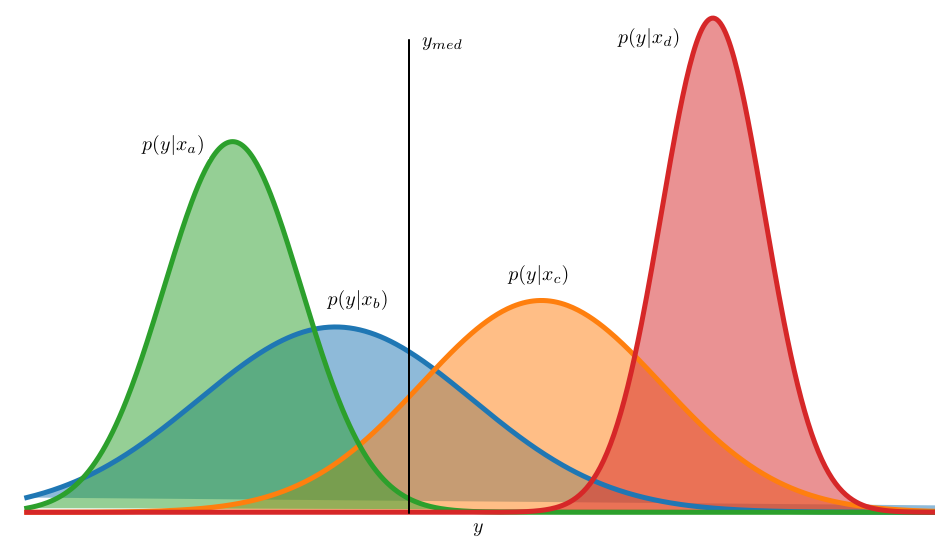
\includegraphics[width=\textwidth]{Img/MostLikelyProba.png}
    \caption{Posibles valores del peso de la bolsa de naranjas y su valor real $y_{med}$}
    \label{fig:mostlikelyproba}
\end{figure}

Tomando en cuenta el modelo de medición presente en la Ecuación (\ref{eq:linearmeasmodel}), el mismo puede ser expresado como una probabilidad condicional de la medición, asumiendo alguna densidad de probabilidad para $v$, por ejemplo, ruido blanco Gaussiano aditivo
\begin{equation}
    v \sim \mathcal{N}(0,\sigma^2)
\end{equation}

entonces, el parámetro desconocido, $x$, resulta ser la media de esta densidad, y la varianza corresponde a la varianza de ruido.
\begin{equation}
    p(y|x) = \mathcal{N}(x,\sigma^2)
\end{equation}

Teniendo en cuenta que la función densidad de probabilidad de una Gaussiana es
\begin{equation}
    \mathcal{N}(z;\mu,\sigma^2) = \frac{1}{\sigma \sqrt{2\pi}} e^{\frac{-(z-\mu)^2}{2\sigma^2}}
\end{equation}

puede expresarse la medición de verosimilitud para una de las mediciones como
\begin{align}
    p(y|x) &= \mathscr{N}(y;x,\sigma^2) \\
           &= \frac{1}{\sqrt{2\pi\sigma^2}} e^{\frac{-(y-x)^2}{2\sigma^2}}
\end{align}

Si se tienen múltiples mediciones múltiples independientes, entonces
\begin{align}
    p(\bm{y}|x) &\propto \mathscr{N}(y_1;x,\sigma^2)\cdot\mathscr{N}(y_2;x,\sigma^2)\cdot...\cdot\mathscr{N}(y_m;x,\sigma^2) \\
            &= \frac{1}{\sqrt{(2\pi)^m\sigma^{2m}}} \exp\left({\frac{-\sum_{i=1}^m(y_i-x)^2}{2\sigma^2}}\right)
\end{align}

El estimador de máxima verosimilitud (MLE) está dado por
\begin{equation}
    \hat{x}_{MLE} = argmax_x p(\bm{y}|x)
\end{equation}

En lugar de tratar de optimizar el verosímil directamente, puede aplicarse el logaritmo
\begin{align}
    \hat{x}_{MLE} = argmax_x \log p(\bm{y}|x)
\end{align}

El logaritmo aumenta monotónicamente. Resulta entonces
\begin{equation}
    \log p(\bm{y}|x) = -\frac{1}{2\sigma^2}\left((y_1-x)^2+...+(y_m-x)^2\right)+C
\end{equation}

Esta ecuación es muy parecida a la suma de los errores cuadráticos. La constante $C$ en esta expresión refiere a términos que no son funciones de $x$ y pueden ser ignorados.

Luego, como el argmax de la función f es equivalente al argmin del negativo de dicha función, 
\begin{equation}
    argmax_z f(z) = argmin_z \left(-f(z)\right)
\end{equation}

el problema del verosímil máximo puede ser escrito como
\begin{align}
    \hat{x}_{MLE} &= argmin_x -\left(\log p(\bm{y}|x)\right) \\
                  &= argmin_x \frac{1}{2\sigma^2}\left((y_1-x)^2+...+(y_m-x)^2\right)
\end{align}

Por lo tanto, es posible realizar la maximización de la verosimilitud mediante una minimización de la suma de errores cuadráticos. Esto es válido ya que se asume que las mediciones se encuentran corrompidas por ruido blanco Gaussiano independiente aditivo de igual varianza.

Finalmente, si se asume que cada medición tiene una varianza distinta, se llega al mismo criterio que en cuadrados mínimos ponderados
\begin{equation}
    \hat{x}_{MLE} = argmin_x \frac{1}{2}\left(\frac{(y_1-x)^2}{\sigma_1^2}+...+\frac{(y_m-x)^2}{\sigma_m^2}\right)
\end{equation}

Resumiendo, en ambos casos, el estimador de máxima verosimilitud para ruido blanco Gaussiano es equivalente a las soluciones de los cuadrados mínimos ordinarios o ponderados.
\begin{equation}
    \hat{x}_{MLE} = \hat{x}_{LS} = argmin_x\mathscr{L}_{LS}(x) = argmin_x\mathscr{L}_{MLE}(x)
\end{equation}

Esto cobra importancia en sistemas realistas, los cuales presentan una gran cantidad de fuentes de ruido. Recordando el teorema central del límite, que establece que cuando se suman variables aleatorias independientes, su suma normalizada tenedrá a una distribución normal, y teniendo en cuenta que el método de cuadrados mínimos es equivalente a calcular la máxima verosimilitud\footnote{Siempre asumiendo que se está en presencia de ruido blanco Gaussiano aditivo}, es posible calcular el mejor estimador de una forma computacionalmente sencilla.

Sin embargo, una consideración importante a tener en cuenta con el método de cuadrados mínimos es cuando se presenta un valor atípico, esto es, los que se encuentran en las "colas" de la Gaussiana, provocando que el estimador final se aleje del valor verdadero. Por ello es importante cuantificar la distribución de error antes de aplicar ciegamente máxima verosimilitud o cuadrados mínimos.

\subsection{Regresión no lineal}

La regresión lineal es un método poderoso para analizar los datos descriptos por modelos que son lineales en los parámetros. Sin embargo, muchas veces las formas de las curvas que mejor ajustan a los datos obtenidos son no lineales en los parámetros. En estos casos, el modelo de regresión sigue siendo de la misma forma que el de la Expresión (\ref{eq:regressionmodel}), a diferencia de que al menos una de las derivadas de la función de expectativa con respecto a los parámetros depende de al menos uno de los parámetros\footnote{Por ejemplo, si derivo $\theta_1 \theta_2 x_1$ respecto a cualquiera de esos dos parámetros, dicha derivada parcial dependerá del parámetro no derivado}.

Para diferenciar entre modelos lineales y no lineales, los parámetros para este último caso se definen con $\bm{\theta}$,
\begin{equation}
    y_i = f(\bm{x}_i, \bm{\theta}) + v_i
    \label{eq:nonlinearregressionmodel}
\end{equation}

El criterio de error cuadrático para modelos no lineales es uno general, del cual puede derivarse la Expresión (\ref{eq:squarederrorcriterion})
\begin{align}
    \mathscr{S}(\bm{\theta}) &= \sum_{i=1}^n (y_i - f(\bm{x}_i;\bm{\theta}))^2 \\
                   &= (\bm{y} - \bm{f}(\bm{\theta}))^T\bm{R}^{-1}(\bm{y} - \bm{f}(\bm{\theta})) \\
                   &= \bm{y}^T \bm{R}^{-1}\bm{y} - 2\bm{y}^T\bm{R}^{-1}\bm{f}(\bm{\theta}) + \bm{f}(\bm{\theta})^T\bm{R}^{-1}\bm{f}(\bm{\theta})
    \label{eq:generalsquarederrorcriterion}
\end{align}
donde $\bm{f}(\bm{\theta}) = (f_1(\bm{\theta}), f_2(\bm{\theta}), ..., f_n(\bm{\theta}))$ y $f_i(\bm{\theta}) = f(\bm{x}_i;\bm{\theta})$.

A diferencia de la situación de cuadrados mínimos lineales, $\mathscr{S}(\bm{\theta})$ puede tener varios mínimos relativos además del mínimo absoluto $\hat{\bm{\theta}}$. Por ello, si bien el \textit{minimizador global} presentado en la Expresión (\ref{eq:globalminimizer}) es válido para este tipo de modelos, este problema es muy difícil de resolver en general, por lo que se presentan sólo métodos para resolver el problema más simple de encontrar un minimizador local para $f$, un vector de argumento que proporciona un valor mínimo de $f$ dentro de una determinada región cuyo tamaño está dado por $\gamma$, donde $\gamma$ es pequeño y positivo. Entonces, debe cumplirse que

\begin{equation}
    f(\theta^*) \leq f(\theta)\hspace{1cm}\text{para}\hspace{1cm}||\theta - \theta^*|| < \gamma
    \label{eq:localminimizer}
\end{equation}
conocido como el \textit{minimizador local}.

La minimización de $\mathscr{S}$ respecto a sus parámetros debe ser realizada iterativamente.
%El objetivo de cada iteración es encontrar una perturbación $\bm{\delta}$ a los parámetros $\bm{\theta}$ que reduzca $\mathscr{S}$.
Desde un punto inicial $\bm{\theta}_0$, el método produce una serie de vectores $\bm{\theta}_1$, $\bm{\theta}_2$, ..., los cuales se espera que converjan a $\bm{\theta}^*$, un minimizador local para la función dada. La mayoría de los métodos tienen medidas que imponen la \textit{condición descendente}
\begin{equation}
    \bm{f}_{i+1}(\bm{\theta}) < \bm{f}_{i}(\bm{\theta})
    \label{eq:descendingcondition}
\end{equation}

Esto evita la convergencia a un maximizador y también hace menos probable que se converja hacia un punto de silla\footnote{Punto sobre una superficie en el que la pendiente es cero pero no se trata de un extremo local, sino que la elevación es máxima en una dirección y mínima en la dirección perpendicular.}. Si la función dada tiene varios minimizadores, el resultado dependerá del punto de partida $\theta_0$. No se sabe a priori cuál de los minimizadores se encontrarán, por lo que no es necesariamente el minimizador más cercano a $\theta_0$.

En muchos casos, el método produce vectores que convergen hacia el minimizador en dos etapas claramente diferentes. Cuando $\theta_0$ está lejos de la solución, se busca que el método produzca iteraciones que se muevan constantemente hacia $\theta^*$. En esta ''etapa global'' de la iteración, es necesario que los errores no aumenten, excepto en los primeros pasos, es decir
\begin{equation}
    ||e_{k+1}|| < ||e_k||\hspace{1cm}\text{para}\hspace{1cm}k<K
\end{equation}
donde $e_k$ responde a la función de error
\begin{equation}
    e_k = \theta_k - \theta^*
\end{equation}

En la etapa final de la iteración, donde $\theta_k$ es cercano a $\theta^*$, se quiere una convergencia más rápida. A partir de esto pueden distinguirse tres casos
\begin{itemize}
    \item \textit{Convergencia lineal}
    \begin{equation}
            ||e_{k+1}|| \leq a||e_k||\hspace{1cm}\text{cuando $||e_k||$ es pequeño}\hspace{1cm}0<a<1
    \end{equation}
    \item \textit{Convergencia cuadrática}
    \begin{equation}
        ||e_{k+1}||=O(||e_k||^2)\hspace{1cm}\text{cuando $||e_k||$ es pequeño}
    \end{equation}
    \item \textit{Convergencia superlineal}
    \begin{equation}
        \frac{||e_{k+1}||}{||e_k||}\rightarrow 0\hspace{1cm}\text{para $k\rightarrow 0$}
    \end{equation}
\end{itemize}

Estos métodos presentados son \textit{métodos de descenso} que satisfacen la condición descendiente de la Expresión (\ref{eq:descendingcondition}) en cada paso de la iteración. Un paso del iterador actual consiste en
\begin{itemize}
    \item Encontrar una \textit{dirección de descenso} $\bm{\delta}_d$, el cual lo será para $\bm{f}$ en $\bm{\theta}$ si $\bm{\delta}^T\bm{f}'(\bm{\theta}) < 0$. En caso de no existir $\bm{\delta}$, entonces $\bm{f}'(\bm{\theta}) = 0$, representando en este caso que $\bm{\theta}$ es estacionario.
    \item Si existe $\bm{\delta}$, hallar una longitud de paso que de una buena disminución en el valor $\bm{f}$ en la dirección dada por $\bm{\delta}_d$, con tal de obtener una disminución en el valor de la función objetivo.
\end{itemize}

Una forma de hacer esto mediante el proceso llamado \textit{búsqueda de línea}, el cual consiste en hallar una aproximación a
\begin{equation}
    \alpha_e = argmin_{\alpha > 0} \bm{f}(\bm{\theta}+\alpha \bm{\delta})
\end{equation}

\subsubsection{Método de descenso de gradiente}

El método de descenso de gradiente es un método de minimización general que actualiza los valores de los parámetros en la dirección de descenso más pronunciada, esto es, la dirección opuesta al gradiente de la función objetivo. El método de descenso de gradiente converge bien para problemas con funciones objetivas simples. Para problemas con muchos parámetros, este método es a veces la única opción viable.

Volviendo al caso de la Expresión (\ref{eq:generalsquarederrorcriterion}), el gradiente de dicha función con respecto a los parámetros es
\begin{align}
    \frac{\partial \mathscr{S}}{\partial \bm{\theta}}\bigg\rvert_{\bm{\theta}=\hat{\bm{\theta}}} &= 2(\bm{y} - \bm{f}(\hat{\bm{\theta}}))^T \bm{R}^{-1}\frac{\partial}{\partial \bm{\theta}}(\bm{y} - \bm{f}(\hat{\bm{\theta}}) \\
    &= -2(\bm{y} - \bm{f}(\hat{\bm{\theta}}))^T \bm{R}^{-1}\left[\frac{\partial \bm{f}(\hat{\bm{\theta}})}{\partial \hat{\bm{\theta}}}\right] \\
    &= -2(\bm{y} - \bm{f}(\hat{\bm{\theta}}))^T \bm{R}^{-1}\bm{J}
\end{align}
donde la \textit{matriz Jacobiana} $\bm{J}$ representa la sensibilidad local de la función $\bm{f}$ a variaciones de los parámetros $\hat{\bm{\theta}}$. Tener en cuenta que en los modelos que son lineales en los parámetros, $\bm{f} = \bm{X}\bm{\theta}$, el Jacobiano es la matriz de los vectores base del modelo, $\bm{X}$. La actualización de parámetros $\bm{\delta}$ que mueve los parámetros en la dirección del \textit{descenso más pronunciado} viene dada por
\begin{equation}
    \bm{\delta}_{gd} = \alpha\bm{J}^T\bm{R}^{-1}(\bm{y} - \bm{f}(\hat{\bm{\theta}}))
\end{equation}
donde el escalar positivo $\alpha$ determina la longitud del escalón en la dirección de descenso más pronunciada.

\subsubsection{Método de Gauss-Newton}
El método de Gauss-Newton es un método para minimizar una función objetivo de suma de cuadrados. Presume que la función objetivo es aproximadamente cuadrática en los parámetros cercanos a la solución óptima. Para problemas de tamaño moderado, el método de Gauss-Newton generalmente converge mucho más rápido que el método de descenso de gradiente.

La función evaluada con parámetros de modelo perturbados puede aproximarse localmente a través de una expansión de la serie Taylor de primer orden.
\begin{equation}
    \bm{f}(\hat{\bm{\theta}+\bm{\delta}}) \approx \bm{f}(\hat{\bm{\theta}}) + \left[\frac{\partial \bm{f}}{\partial \hat{\bm{\theta}}}\right]\bm{\delta} = \bm{f}(\hat{\bm{\theta}}) + \bm{J}\bm{\delta}
    \label{eq:gaussnewtontaylor}
\end{equation}

Substituyendo la Expresión (\ref{eq:gaussnewtontaylor}) en (\ref{eq:generalsquarederrorcriterion}) para $\mathscr{S}(\bm{\theta} + \bm{\delta})$
\begin{equation}
    \begin{aligned}
        \mathscr{S}(\bm{\theta}+\bm{\delta}) \approx{} &\bm{y}^T\bm{R}^{-1}\bm{y} + \bm{f}(\bm{\theta})^T\bm{R}^{-1}\bm{f}(\bm{\theta}) - 2\bm{y}^T\bm{R}^{-1}\bm{f}(\bm{\theta}) - \\
        & -2\left(\bm{y} - \bm{f}(\bm{\theta})\right)^T\bm{R}^{-1}\bm{J}\bm{\delta} + \bm{\delta}^T\bm{J}^T\bm{R}^{-1}\bm{J}\bm{\delta}
    \end{aligned}
\end{equation}
La aproximación de Taylor de primer orden  de la Expresión (\ref{eq:gaussnewtontaylor}) da como resultado una aproximación para $\mathscr{S}$ que es cuadrática en $\bm{\delta}$. Por lo tanto, el $\bm{\delta}$ que minimiza a $\mathscr{S}$ se encuentra cuando $\frac{\partial \mathscr{S}}{\partial \bm{\delta}} = 0$
\begin{equation}
    \frac{\partial}{\partial \bm{\delta}}\mathscr{S}(\bm{\theta} + \bm{\delta}) \approx -2\left(\bm{y} - \bm{f}(\bm{\theta})\right)^T\bm{R}^{-1}\bm{J} + 2\bm{\delta}^T\bm{J}^T\bm{R}^{-1}\bm{J}
\end{equation}
y las ecuaciones normales resultantes para la actualización de Gauss-Newton son
\begin{equation}
    \left[\bm{J}^T\bm{R}^{-1}\bm{J}\right]\bm{\delta}_{gn} = \bm{J}^T\bm{R}^{-1}(\bm{y} - \bm{f}(\bm{\theta})
\end{equation}

\subsubsection{Método de Levenberg-Marquardt}
El algoritmo de Levenberg-Marquardt varía adaptativamente las actualizaciones de parámetros entre la actualización de descenso de gradiente y la actualización de Gauss-Newton,
\begin{equation}
    \left[\bm{J}^T\bm{R}^{-1}\bm{J} + \lambda\bm{I}\right]\bm{\delta}_{lm} = \bm{J}^T\bm{R}^{-1}\left(\bm{y} - \bm{f}(\bm{\theta}\right)
\end{equation}{}
donde pequeños valores del \textit{parámetro de amortiguación} $\lambda$ resultan en una actualización de Gauss-Newton, mientras que valores grandes de $\lambda$ llevan a una actualización de descenso de gradiente. El parámetro de amortiguación $\lambda$ se inicializa para que sea grande, de modo que las primeras actualizaciones sean pequeños pasos en la dirección de descenso más pronunciada. Si alguna iteración resulta en una peor aproximación $(\mathscr{S}(\bm{\theta} + \bm{\delta}_{lm}) > \mathscr{S}({\bm{\theta}}))$, entonces $\lambda$ se aumenta. De lo contrario, a medida que la solución mejora, $\lambda$ disminuye, haciendo que el método de Levenberg-Marquardt se aproxima al método de Gauss-Newton, y la solución generalmente se acelera al mínimo local.

En la relación de actualización de Marquardt
\begin{equation}
    \left[\bm{J}^T\bm{R}^{-1}\bm{J} + \lambda\;  diag(\bm{J}^T\bm{R}^{-1}\bm{J})\right]\bm{\delta}_{lm} = \bm{J}^T\bm{R}^{-1}\left(\bm{y} - \bm{f}(\bm{\theta})\right)
\end{equation}{}
los valores de $\lambda$ se normalizan a los valores de $\bm{J}^T\bm{R}^{-1}\bm{J}$.

En sistemas donde solo hay un mínimo, el método de Levenberg-Marquardt convergerá al mínimo global incluso si la suposición inicial es arbitraria. En cambio, en sistemas con mínimos múltiples, es más probable que el método encuentre el mínimo global si la suposición inicial ya está cerca de la solución. Sin embargo, el mismo permite que la selección de valores iniciales esté más lejos de la solución que el método de Gauss-Newton.

Si bien existen numerosas implementaciones de este método, se presentará a continuación la solución propuesta por la \textit{librería Eigen}.

\newpage
\section{Simultaneous Localization And Mapping}
\label{sec:slam}
Esta sección describe los conocimientos básicos respecto a la Localización y Mapeo Simultáneos (SLAM), a la vez de introducir parte de los algoritmos y sensores mencionados en secciones anteriores. Si se quiere profundizar más en el tema se recomienda consultar \textbf{(Suenderhauf, 2012)(Reid, 2016)}.

\subsection{Introducción al SLAM}
El problema de localización y mapeo simultáneos (SLAM) se basa en el proceso de un robot que construye un mapa de su entorno desconocido (\textit{mapping}) mientras este lo explora conociendo su ubicación en el mismo (\textit{localization}). Dicho problema puede ser expresado como el dilema del huevo o la gallina, ya que para conocer la ubicación del robot, es necesario determinar el mapa que lo rodea, sin embargo, para que el mismo pueda estimar el mapa en el cual se encuentra, necesita primero conocer su ubicación dentro de ese entorno. 

A partir de la detección y seguimiento de marcas naturales del ambiente (\textit{landmarks}), las técnicas de SLAM  estiman  tanto  la  posición  del  robot  como  la  ubicación  de las marcas en el entorno. El mapa se construye con las estimaciones de las posiciones  de  dichas  marcas,  las  cuales  van  siendo ajustadas  a  medida  que  son observadas desde distintas posiciones. Es necesario que la localización sea precisa, ya que si la misma es inexacta generará problemas a la hora de reconstruir el mapa. Es por esto que el mapeo y la localización dependen uno del otro, y se ejecutan \textit{simultáneamente} de forma entrelazada.

El SLAM es un problema difícil ya que, debido al ruido de los sensores utilizados, ninguna de las mediciones es perfecta. Esto significa que ni el movimiento del robot ni la estructura del entorno se conocen de manera absolutamente precisa, sino solo hasta cierto grado de incertidumbre. Con el fin de hacer frente a estas incertidumbres, el SLAM generalmente se entiende y se aborda mediante técnicas y modelos probabilísticos. Las diferentes formas en que se representan las funciones de densidad probabilística constituyen las diferencias en cada enfoque. 
\textbf{MIRAR LO COMENTADO}
% Muchas de ellas utilizan filtros de Bayes, tal como lo es el Filtro de Kalman Extendido (EKF) 
% \begin{large}
% [DURRANT-WHYTE2006]
% [KALMAN1960]
% \end{large}, o en versiones más modernas, por ejemplo, el Fast-SLAM
% \begin{large}
% [PONER FASTSLAM BIEN]
% \end{large}. 
Sin embargo, el uso de enfoques de estimación de estado para describir el problema de SLAM implica resolver una serie de inconvenientes que se generan a partir del mismo, siendo de los más destacados la \textit{asociación de datos}\textbf{[ref 103 y 104 de reid2016]} y el \textit{cierre de ciclo}.

\subsubsection{Asociación de datos}
Uno de los problemas comunes dentro del SLAM corresponde a la asociación de datos (\textit{data asociation}), el cual es el proceso de asociar los datos de los sensores utilizados con las características del ambiente, generando de esta forma los landmarks. En otras palabras, se busca asociar la medición del sensor con alguno de los \textit{n} landmarks ya extraídos y, en caso de que no pertenezca a ninguno de ellos, se generará un landmark nuevo \textit{n+1}. Es importante poder discernir de cuál landmark se trata o si es en efecto uno nuevo, ya que debido al ruido inherente de los sensores puede que caiga entre dos de ellos, como puede observarse en la Figura \ref{fig:dataassociation}, haciendo que pueda tender equívocamente al incorrecto, o creer que no se tiene dicho landmark cuando en realidad era uno ya medido.

\begin{figure}[!ht]
    \centering
    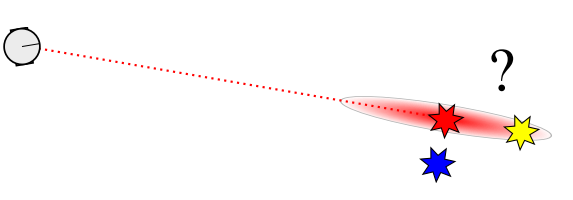
\includegraphics[width=\textwidth]{Img/DataAssociation.png}
    \caption{El problema de la asociación de datos: dificultad de discernir si el landmark detectado (rojo) corresponde a alguno de los ya existentes, o si en realidad es uno del que no se tuvo registro anteriormente}
    \label{fig:dataassociation}
\end{figure}

\subsubsection{Online SLAM y full SLAM}
Los mapas SLAM se construyen a partir de millones de lecturas de sensores, que se comparan entre sí en un paso de asociación de datos que depende completamente de las estimaciones de pose actuales. Para este caso, en el que tanto la pose como el mapa se expresan sólo en base a las mediciones del paso de tiempo actual, el problema se lo conoce como \textit{online SLAM} y se expresa mediante el posterior
% \bm{p}_t es la pose y m el mapa. z es la medicion y u la variable de control
% seria el maximum likelihood?
\begin{equation}
    p(\bm{p},\bm{m}|\bm{y}_{0:t},\bm{u}_{0:t})
\end{equation}
siendo $\bm{p}$ la pose, $\bm{m}$ el mapa, $\bm{y}$ las mediciones y $\bm{u}$ las variables de control.

En cambio, la evaluación y la reevaluación de estas asociaciones de datos, al mismo tiempo que se calcula y actualiza \textit{todo el historial} de poses del robot, describe el problema de \textit{full SLAM} \textbf{[ref 6 de reid2016]}
\begin{equation}
    p(\bm{p}_{0:t},\bm{m}|\bm{y}_{0:t},\bm{u}_{0:t})
\end{equation}

Si bien este último no puede resolverse para entornos no triviales, los enfoques descritos en la literatura a menudo producen resultados útiles en entornos del mundo real. En concreto, con el fin de reducir la complejidad del algoritmo se toman como supuestos comunes que el \textit{entorno es estático}, es decir, que el mapa no varía con el tiempo, y por segundo que las trayectorias de los robots \textit{pueden predecirse}, logrando así que los modelos de movimiento puedan predecir dónde es probable que esté un robot, permitiendo que la búsqueda de asociaciones de datos comience cerca del óptimo global.

\subsubsection{Cierre de ciclo}
\textbf{[REFS DE REID Y VER CASTRO]}
Si bien lo que se busca es evitar errores principalmente de localización, debido al ruido inherente de los sensores utilizados como se mencionó anteriormente, los algoritmos de SLAM no pueden estimar exactamente tanto la ubicación del robot como el mapa que lo rodea, sino hasta con cierto grado de incertidumbre. Como se ejecuta el algoritmo de manera secuencial, el error se irá acumulando a través del tiempo, resultando en una pésima estimación luego de varias corridas. Una forma de poder mitigar en parte estos errores es mediante el reconocimiento de una posición en la que el robot ya estuvo anteriormente. Tomar conocimiento de que se ha efectuado un ciclo en la trayectoria permite calcular el error cometido en la estimación de la posición y da origen a una serie de procesos que permiten corregir tanto la localización actual del robot como el mapa hasta ese momento construido. Este reconocimiento se lo conoce como \textit{cierre de ciclo} (\textit{loop closure}), el cual puede verse en la Figura \ref{fig:poseloopclcorr}.


\begin{figure}[!ht]
    \centering
    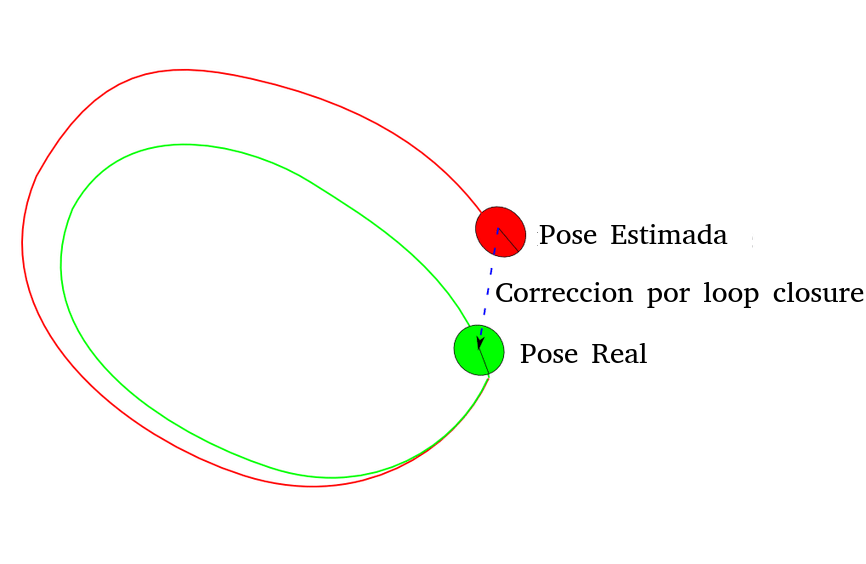
\includegraphics[width=\textwidth]{Img/Pose_LoopClosureCorr.png}
    \caption{Estimación de pose y su correción mediante el loop closure}
    \label{fig:poseloopclcorr}
\end{figure}

% \ifslamext
\subsection{Mapas}
\textbf{DE Suenderhauf 2012}
En base a los sensores extereoceptivos utilizados además del entorno en el que se encuentran los robots y tareas que tengan que realizar, los mapas creados pueden variar considerablemente. \textbf{THRUN 2002, SICILIANO 2008, THRUN 2005} A continuación, se presentan dos tipos de mapas que pueden encontrarse en la literatura.

\subsubsection{Occupancy Grid Maps}
El concepto de esta técnica es la de discretizar el ambiente a mapear, utilizando pequeñas celdas o regiones discretas $m_i$, como puede observarse en la Figura \ref{fig:occupancygridmaps}.a. A cada una de estas celdas se le asocia un valor que expresa la probabilidad
\begin{equation}
    p(m_i|\bm{y}_{0:t},\bm{x}_{0:t})
\end{equation}
de que dicha celda esté ocupada por un obstáculo, dados todos los datos de los sensores hasta el momento ($\bm{y}_{0:t}$) y todas las poses del robot ($\bm{x}_{0:t}$). En caso de que se desconozca el valor de dichas celdas, el valor por defecto de las mismas es de 0.5. 

\begin{figure}[!ht]
    \centering
    \subfloat[Representación de cada celda en base a si la misma se encuentra ocupada, libre o no se tiene información al respecto]{{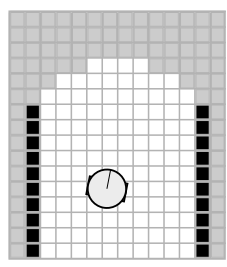
\includegraphics[width=0.45\textwidth]{Img/OccupancyGrids.png}}}%
    \qquad
    \subfloat[Mapa generado por un LIDAR]{{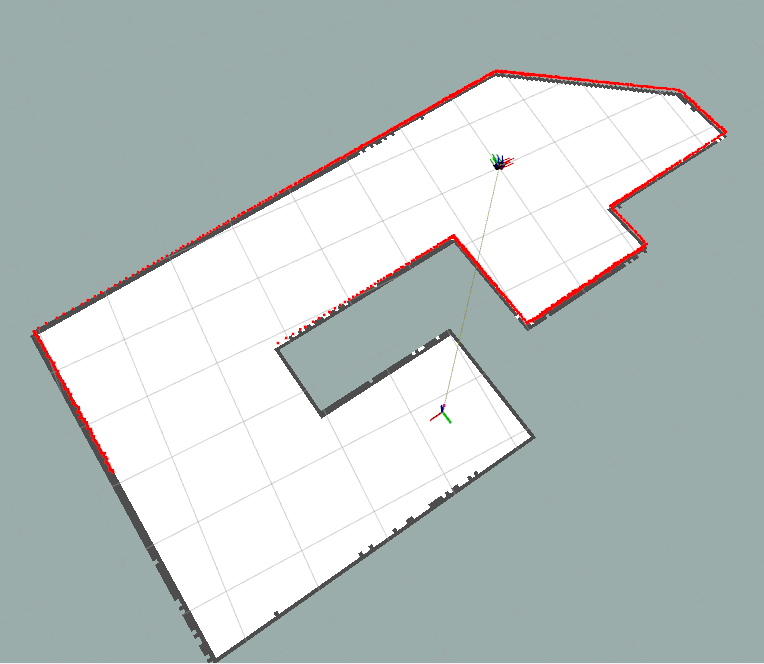
\includegraphics[width=0.45\textwidth]{Img/LIDAROccupancyGridMap.png}}}%
    \caption{Occupancy Grid Maps}
    \label{fig:occupancygridmaps}
\end{figure}


Un ejemplo de un mapa generado por un LIDAR 2D puede observarse en la Figura \ref{fig:occupancygridmaps}.b, donde los cuadros blancos corresponden a celdas libres, los negros a las ocupadas y, las grises, a las que no se tiene información alguna. A su vez, estos mapas pueden llevarse a la espacio tridimensional para representar datos provenientes de, por ejemplo, LIDAR 3D o cámaras.

\subsubsection{Mapas de características}
A diferencia de los Occupancy Grid Maps, los cuales generan un mapa denso del ambiente, los \textit{mapas de características} contienen sólo la posición de distintos landmarks o características del ambiente, resultando en un mapa disperso. Un ejemplo del mismo puede verse en la Figura \ref{fig:dataassociation} \textbf{O PONGO OTRA IMG?}. Dependiendo del principio de medición del sensor que recolecta estos landmarks, existen diferentes tipos de ellos
\begin{itemize}
    \item \textit{El Rango y el rumbo} se conocen, tal como es el caso de las cámaras estéreo o las cámaras RGB-D, en el que la ubicación del landmark respecto al sensor se encuentra bien definida, resultando ser el más sencillo de los tres tipos. En la Figura \ref{fig:landmarktypes}.a puede observarse al mismo.
    \item \textit{Sólo el rango} es conocido, como se observa en la Figura \ref{fig:landmarktypes}.b, haciendo que sea necesario triangular, por ejemplo, para la señal de WiFi, entre la fuerza de la señal recibida de diferentes routers y así conseguir la ubicación del robot en base a estos.
    \item \textit{Sólo el rumbo} es conocido, observado en la Figura \ref{fig:landmarktypes}.c, como es el caso de las cámaras monoculares, haciendo difícil medir la profundidad de cada punto.
\end{itemize}

\begin{figure}[!ht]
    \centering
    \subfloat[Se tiene rango y rumbo]{{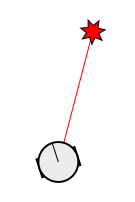
\includegraphics[width=0.3\textwidth]{Img/LandmarkRangeBearing.png}}}%
    \qquad
    \subfloat[Se tiene sólo el rango]{{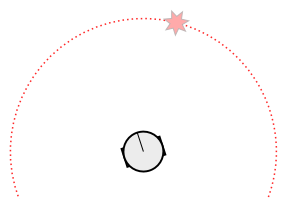
\includegraphics[width=0.3\textwidth]{Img/LandmarkRange.png}}}%
    \subfloat[Se tiene sólo el rumbo]{{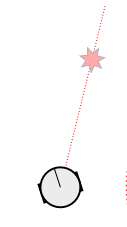
\includegraphics[width=0.3\textwidth]{Img/LandmarkBearing.png}}}%
    \caption{Tipos de landmarks}
    \label{fig:landmarktypes}
\end{figure}

% \subsubsection{Grafos de pose}
% Los grafos de pose representan la trayectoria del robot como una estructura grafos donde los nodos representan las poses del robot y los bordes entre los nodos representan las conexiones espaciales entre estas poses. Los bordes contienen, por ejemplo, información de odometría o expresan cierres de ciclo. En la Figura puede verse el esquema de un grafo de pose, donde la trayectoria del robot es representada por los grafos donde los nodos son las poses del robot en un punto concreto de tiempo.
% \begin{figure}[!ht]
%     \centering
%     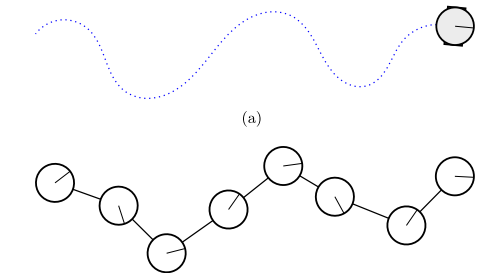
\includegraphics[width=\textwidth]{Img/PoseGraphStructure.png}
%     \caption{Esquema de un grafo de pose}
%     \label{fig:posegraphstructure}
% \end{figure}

% Si bien los landmarks explícitos u otra información sobre el medio ambiente no son parte del grafo de pose en sí, dicha información se puede adjuntar a los nodos en el grafo, lo que permite que el grafo de pose exprese occupancy grids en 2D o 3D o mapas de características y cualquier combinación de ellos.

\ifimagenes
\else
\subsection{Algoritmos de SLAM}
Puede decirse que un algoritmo de SLAM consiste en tres operaciones básicas, las cuales se repiten en cada paso de tiempo
\begin{itemize}
    \item El robot se mueve por el entorno, hasta alcanzar un nuevo punto de vista de la escena, que debido al ruido inherente de los sensores ocasiona que aumente la incertidumbre en la localización del mismo.
    \item El robot descubre landmarks en el ambiente, los que requieren ser incorporados al mapa.
    \item El robot observa el mapa que fue mapeado anteriormente y lo utiliza para corregir tanto la localización de dicho landmark como la del propio robot.
\end{itemize}

Si bien existen numerosos algoritmos para realizar el problema de SLAM, a continuación se describen dos de los enfoques que se encuentran en la literatura respecto al tema en cuestión.

\subsubsection{EKF-SLAM}
El enfoque del EKF para solucionar el problema de SLAM se trata de un problema orientado al online SLAM mediante el uso de datos de sensores recopilados a partir del movimiento y la rotación del robot. Esto se puede hacer, por ejemplo, utilizando encoders y una IMU. Además, también es necesario recopilar información del entorno mediante, por ejemplo, el uso de un LIDAR. Con estos datos, el algoritmo realiza un seguimiento del lugar donde probablemente se ubica el robot dentro de un mapa, así como un seguimiento de los puntos de referencia específicos observados. Es por esto que se utiliza un mapa de características para este caso.

Al considerar un mapa estático, el único factor variante en el tiempo es el movimiento del robot. Por lo tanto, se tienen diferentes comportamientos para cada parte del vector de estados. El mismo en este caso se define como
\begin{equation}
    \bm{x} = 
    \begin{bmatrix}
        \bm{p} \\
        \bm{\mathcal{M}}
    \end{bmatrix}
\end{equation}
donde $\bm{p}$ corresponde a la pose del robot\footnote{Por lo general se suele incorporar la velocidad, ya que se utilizan las ecuaciones de la física clásica. Para la orientación puede utilizarse la forma de cuaterniones mediante la Expresión (\ref{eq:edoquaternion}).} y $\bm{\mathcal{M}}=(\mathcal{L}_1,...,\mathcal{L}_n)$ corresponde a los estados de los landmarks, siendo $n$ la cantidad de ellos detectados. En base a este, el resto de los parámetros del filtro de Kalman Extendido se modificarán respecto al visto en la Sección \ref{sec:stateestimation}\textbf{[SOLA 2014]}. Puede verse que a medida que el mapa aumenta, el costo computacional se incrementará, ya que se tendrán cada vez más landmarks.

Además de la complejidad cuadrática, este filtro cuando se aplica al problema SLAM tiene como desventaja sustancial \textbf{[Csorba 1997 DE SU - FAST-SLAM]}
la sensibilidad a fallas que presenta en las asociaciones de datos. Este problema con el EKF se aplica en situaciones en las que se desconocen las asociaciones de datos. El EKF mantiene una única hipótesis de asociación de datos por observación, típicamente elegida usando una heurística de máxima verosimilitud. Si la asociación de datos elegida por esta heurística es incorrecta, el efecto de incorporar esta observación en el EKF nunca se puede eliminar.

% \subsubsection{FastSLAM}


\subsubsection{GraphSLAM}
Utilizando un grafo de poses, el GraphSLAM se orienta a un problema de full SLAM que consta de dos restricciones. Primero, necesita de datos de odometría (que suelen ser las entradas de control $\bm{u}$) que conecten los estados de las poses $\bm{x}_k$ y $\bm{x}_{k+1}$ como puede ser mediante los datos de un LIDAR o la odometría propia de los encoders
\begin{equation}
    \bm{x}_{k+1} \sim \mathcal{N}(f(\bm{x}_{k},\bm{u}_k),\bm{R}_k)
\end{equation}
donde $\bm{\Sigma}_k$ corresponde a la matriz covarianza en el paso de tiempo $k$.

Segundo, para poder detectar un cierre de ciclo, dos poses, que pueden no ser contiguas, se conectan mediante una Gaussiana,
\begin{equation}
    \bm{x}_j \sim \mathcal{N}(f(\bm{x}_k,\bm{c}_{kj}), \bm{Q}_{kj})
\end{equation}
siendo $\bm{c}_{kj}$ el cierre de ciclo.

La solución para este tipo de SLAM se basa en el método del máximo a posteriori (MAP), siendo $\bm{x}^*$ el punto donde la distribución tiene su máximo
\begin{equation}
    \bm{x}^* = argmax_x\ p(\bm{x}|\bm{u})
\end{equation}

Siendo que tanto la odometría como el cierre de ciclo cuentan con distribuciones Gaussianas independientes, el posterior puede factorizarse como
\begin{equation}
    p(\bm{x}|\bm{u},\bm{c}) \propto \underbrace{\prod_k p(\bm{x}_{k+1}|\bm{x}_{k},\bm{u}_k)}_{\text{\parbox{10em}{\centering Restricciones de odometría}}}\ \underbrace{\prod_{kj}p(\bm{x}_j|\bm{x}_k,\bm{c}_{kj})}_{\text{\parbox{10em}{\centering Restricciones de cierres de ciclo}}}
\end{equation}
que, aplicando el logaritmo como en la Expresión (\ref{eq:mlewithlog}), y teniendo en cuenta la analogía con los cuadrados mínimos ponderados
\begin{align}
    \bm{x}^* &= argmax_x\ p(\bm{x}|\bm{u},\bm{c}) \\
    &= argmin_x\ -log(\bm{x}|\bm{u},\bm{c}) \\
     &= argmin_x\ \bm{e}_k^T\bm{R}_k^{-1}\bm{e}_k + \bm{e}_{kj}^T\bm{Q}_{kj}\bm{e}_{kj} \\
     &= argmin_x\ \underbrace{\sum_{i} ||f(\bm{x}_i,\bm{u}_i)-\bm{x}_{i+1})||^2_{\bm{R}_i}}_{\text{{\centering Restricciones de odometría}}} + \underbrace{\sum_{kj} ||f(\bm{x}_i,\bm{c}_{kj}) - \bm{x}_{j}||^2_{\bm{Q}_{kj}}}_{\text{{\centering Restricciones de cierres de ciclo}}}
\end{align}
siendo $||a-b||^2_{\bm{O}} = (a - b)^T\bm{O}^{-1}(a-b)$ la definición de la distancia Mahalanobis. Esta puede minimizarse con algunas de las regresiones vistas en la Sección \ref{sec:regressionanalysis}, dependiendo de la morfología de la señal $f$.

\fi

% \fi

\subsection{Resumen}
En esta Sección se presentaron algunos conceptos importantes referidos a SLAM, los cuales serán abordados en secciones posteriores.

\newpage
\section{Plataformas disponibles}

En esta sección se evaluarán principalmente diferentes plataformas de hardware disponibles en el mercado\footnote{El relevamiento fue realizado en la fecha 7 de Julio de 2018}. Si bien muchos autores han desarrollado arquitecturas de robots capaces de localización y mapeo simultáneos (SLAM) \cite{engel2012}, \cite{engel2014}, \cite{hausman2016}, las plataformas de control de las mismas no cuentan con un factor de forma de hardware definido que, si bien la cantidad de trabajos que lo utilizan son acotados \cite{qi2009}, esto permite la interconexión de la placa base con nuevos módulos a elegir por el usuario de la plataforma, logrando así expandir sus funcionalidades.

\subsection{Plataformas basadas en FPGA}
\begin{itemize}
    \item \textbf{Phenix Pro DevKit:} está diseñado sobre un System on Chip (SoC) por RobSense Tech, es reconfigurable. El controlador de vuelo (Fig. \ref{fig:fpga_based}.a) incluye el sistema operativo en tiempo real basado en FreeRTOS (UOS) y un Robot Operating System (ROS) basado en Linux. Esta plataforma soporta mas de 20 interfaces incluyendo sensores on-board, mmWave radar, Lidar, entre otros. Permite visión artificial y aplicaciones de algoritmos de Deep Neural Networks \cite{shah2017}.
    
    \item \textbf{Octagonal Pilot on Chip (OcPoc):} desarrollado por Aerotenna Company (Fig. \ref{fig:fpga_based}.b), expande sus capacidades entradas y salidas al incluir pines completamente programables de PWM, PPM y GPIO para integrar con un gran número de diferentes sensores adicionales. Incluye además otros conectores estándar para periféricos tales como GPS y tarjeta SD. El mismo corre la plataforma de software Autopilot \cite{autopilot} e implementa un procesamiento simultáneo, en tiempo real, de los datos de los sensores.
    \begin{figure}[!ht]
        \centering
        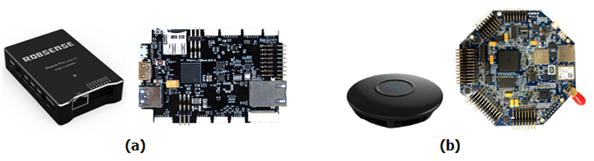
\includegraphics[width=.95\textwidth]{Img/fpga_based}
        \caption{Controlador de vuelo: (a) Phoenix Pro DevKit, (b) OcPoc}
        \label{fig:fpga_based}
    \end{figure}
\end{itemize}

\subsection{Plataformas basadas en ARM MCUs}
\begin{itemize}
    \item \textbf{Pixhawk:} consiste en un controlador PX4-Flight Management Unit (FMU) y una PX4-IO integrada en una misma placa con IO adicionales, memoria y otras características (Fig. \ref{fig:pixhawks}.a). Se encuentra dentro del proyecto DroneCode [REF DRONECODE].
    \item \textbf{Pixhawk 2:} Es un cubo pequeño que cuenta con tres IMUs redundantes y hasta tres módulos GPS (Fig. \ref{fig:pixhawks}.b) (Ardupilot). Toda la conección IO del cubo se encuentra en un conector DF17. Su placa portadora posee una interfaz con Intel Edison.
    
    \begin{figure}[!ht]
        \centering
        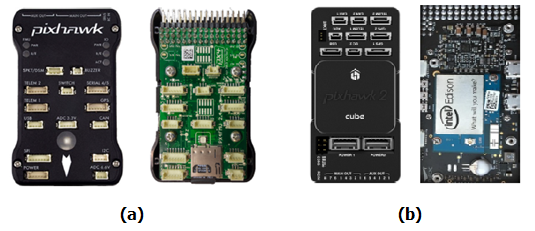
\includegraphics[width=.95\textwidth]{Img/pixhawks}
        \caption{Controlador de vuelo: (a) Pixhawk, (b) Pixhawk 2}
        \label{fig:pixhawks}
    \end{figure}
    
    \item \textbf{FlightCtrl:} Desarrollada por MikroKopter, su última versíon introducida al mercado, la V3.0 (Fig. \ref{fig:flypaparazzi}.a), cuenta con un microcontrolador avanzado, sistema de telemetría, GPS, entre otros, además de ofrecer sistemas con placas de control de vuelo duplicadas que mantienen el helicóptero estable incluso si hay una falla en la placa primaria de control de vuelo.
    \item \textbf{Paparazzi:} Es el primer proyecto de software y hardware open-source para drones [Brisset]. En marzo de 2017 salió el nuevo autopilot del mismo llamado Chimera (Fig. \ref{fig:flypaparazzi}.b) el cual está basado en el microcontrolador STM32F7.
    \item \textbf{FlyMaple:} basada en el Maple Project, el cual es un procesador Arduino ARM, consiste en una placa controladora para cuadricópteros (Fig. \ref{fig:flypaparazzi}.c). La misma cuenta como aplicaciones típícas las de robots balancines, plataformas móbiles, helicópteros y cuadricópteros que requieren IMUs y controladores en tiempo real de alto rendimiento.
    
    \begin{figure}[!ht]
        \centering
        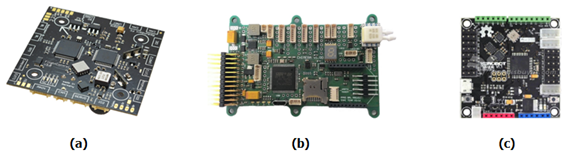
\includegraphics[width=.95\textwidth]{Img/flypaparazzi}
        \caption{Controlador de vuelo: (a) FlightCtrl v3.0, (b) Paparazzi Chimera, (c) FlyMaple}
        \label{fig:flypaparazzi}
    \end{figure}
    
    \item \textbf{CC3D y Atom:} Son dos controladoras de vuelo que poseen las mismas funcionalidades pero con tamaños diferentes. Los mismos (Figs. \ref{fig:apmatom}.a y \ref{fig:apmatom}.b) tienen todos los tipos de hardware de estabilización que corre el firmware OpenPilot/LibraPilot. Pueden ser configuradas para volar con cualquier frame.
    
    \item \textbf{Ardupilot Mega (APM):} Desarrollada por la comunidad DIY Drones como una mejora de la controladora de vuelo Autopilot, consiste en una plataforma basada en  el Arduino Mega (Fig. \ref{fig:apmatom}.c). Puede controlar multicópteros autónomos, helicópteros tradicionales, entre otros.

    \begin{figure}[!ht]
        \centering
        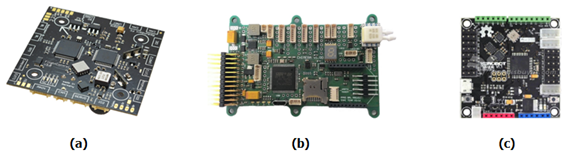
\includegraphics[width=.95\textwidth]{Img/flypaparazzi}
        \caption{Controlador de vuelo: (a) CC3D, (b) Atom, (c) Ardupilot Mega 2.8}
        \label{fig:apmatom}
    \end{figure}
\end{itemize}

\subsection{Plataformas basadas en Raspberry Pi}
\begin{itemize}
    \item \textbf{Erle-Brain 3:} Consiste en un open pilot para drones basado en Linux desarrollado por Erle Robotics (Fig. \ref{fig:raspi}.a) (Erle-Robotics). Combina una Raspberry Pi junto a PXFmini, contando esta última con sensores, IO y alimentación. Está diseñado sobre el proyecto DroneCode.
    \item \textbf{NAVIO2 Autopilot:} Es una integración de sensores, GPS y alimentación apareado con una Raspberry Pi. Cuenta con doble IMU para mejorar el desempeño y conseguir redundancia (Fig. \ref{fig:raspi}.b).
    
    \begin{figure}[!ht]
        \centering
        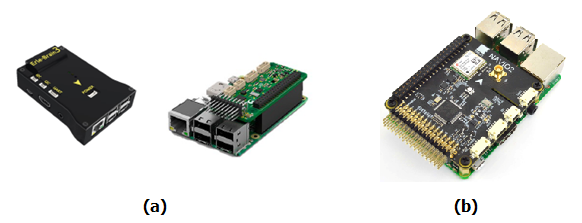
\includegraphics[width=.95\textwidth]{Img/raspi}
        \caption{Controlador de vuelo: (a) Erle-Brain 3 Autopilot, (b) NAVIO2 Autopilot}
        \label{fig:raspi}
    \end{figure}
\end{itemize}

\subsection{Plataformas basadas en Qualcomm}
\begin{itemize}
    \item \textbf{Snapdragon Autopilot:} la plataforma Snapdragon Flight (Fig. \ref{fig:snapdragon}) es un piloto automático de gama alta que puede ejecutar el plan de vuelo sobre un sistema operativo en tiempo real DSP utilizando la API DSPAL para la compatibilidad con POSIX. El mismo cuenta con un SoC Snapdragon 801. En comparación con la Pixhawk, sus características incluyen potencia de procesamiento avanzada, control de vuelo en tiempo real en Hexagon DSP, Wi-Fi, conectividad Bluetooth, GPS automotriz, una cámara de flujo óptico y una cámara de video de resolución 4K.    
    \begin{figure}[!ht]
        \centering
        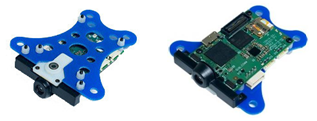
\includegraphics[width=.55\textwidth]{Img/snapdragon}
        \caption{Snapdragon Flight}
        \label{fig:snapdragon}
    \end{figure}
\end{itemize}

\subsection{Comparación entre plataformas existentes}


En el Cuadro \ref{tab:plataformas} (Yang, 2016)(Raj, 2016) se resumen las características principales. En la misma, se observa que la principal diferencia entre ellas es la unidad de procesamiento, además de que no todas ellas presentan redundancia de sensores críticos.

% Please add the following required packages to your document preamble:
% \usepackage{booktabs}
% \usepackage{graphicx}
\begin{table}
\resizebox{\textwidth}{!}{%
\begin{tabular}{@{}|c|c|c|c|c|c|c|@{}}
\toprule
\textbf{Plataforma} & \textbf{Procesador} & \textbf{Sensores} & \textbf{\begin{tabular}[c]{@{}c@{}}Interfaces /\\ Conectividad\end{tabular}} & \textbf{Redundancia} & \textbf{\begin{tabular}[c]{@{}c@{}}Dimensiones \\ (mm)\end{tabular}} & \textbf{Peso (g)} \\ \midrule
Phoenix Pro & \begin{tabular}[c]{@{}c@{}}Xilinx Zynq\\ 7020\end{tabular} & \begin{tabular}[c]{@{}c@{}}Acelerometro,\\ giroscopo,\\ barómetro,\\ GPS\end{tabular} & \begin{tabular}[c]{@{}c@{}}USB, UART, I2C,\\ CAN, SPI, miniHDMI,\\ Camera Link, LVDS,\\ PWM, telemetria\end{tabular} & - & 73,8*55,8*18 & 64 \\ \midrule
OcPoc & \begin{tabular}[c]{@{}c@{}}Xilinx Zynq\\ Z-7010\end{tabular} & \begin{tabular}[c]{@{}c@{}}IMU 9 DOF\\ (MPU9250),\\ Barometro\\ (MS5611)\end{tabular} & \begin{tabular}[c]{@{}c@{}}I2C, USB-OTG,\\ USB-UART, SPI, \\ CSI, GSI, CAN, \\ ADC, PWM\end{tabular} & \begin{tabular}[c]{@{}c@{}}IMU\\ (MPU9250)\end{tabular} & 92*64*21 & 70 \\ \midrule
PIXHAWK & \begin{tabular}[c]{@{}c@{}}ARM\\ Cortex-M4F\end{tabular} & \begin{tabular}[c]{@{}c@{}}Giroscopo\\ (L3GD20H),\\ acelerometro /\\ magnetometro\\ (LSM303D),\\ barometro\\ (MS5611)\end{tabular} & \begin{tabular}[c]{@{}c@{}}UART, CAN, I2C,\\ SPI, ADC, PWM\end{tabular} & \begin{tabular}[c]{@{}c@{}}Giroscopo /\\ acelerometro \\ (MPU6000)\end{tabular} & 50*15,5*81,5 & 38 \\ \midrule
PIXHAWK2 & \begin{tabular}[c]{@{}c@{}}ARM\\ Cortex-M4F\end{tabular} & \begin{tabular}[c]{@{}c@{}}IMU 9 DOF\\ (MPU9250 /\\ ICM20948 /\\ ICM20648 /\\ L3GD20 +\\ LSM303D), \\ Barometro\\ (MS5611)\end{tabular} & \begin{tabular}[c]{@{}c@{}}S.Bus, I2C, SPI, \\ CAN, Carrier board \\ para Intel\\ Edison, ADC, \\ PWM\end{tabular} & \begin{tabular}[c]{@{}c@{}}2x IMU \\ (MPU9250),\\ Barometro\\ (MS5611)\end{tabular} & \begin{tabular}[c]{@{}c@{}}50*15,5*81,6\\ +35*35 (Cube)\end{tabular} & - \\ \midrule
FlightCtrl V3.0 & \begin{tabular}[c]{@{}c@{}}ARM\\ Cortex-M4F\end{tabular} & \begin{tabular}[c]{@{}c@{}}Giroscopo,\\ magnetometro,\\ acelerometro,\\ barometro, GPS\end{tabular} & \begin{tabular}[c]{@{}c@{}}UART, I2C, SPI, \\ ADC, PWM, S.Bus, \\ CAN, telemetria\end{tabular} & - & 67*67*- & 32 \\ \midrule
Paparazzi & STM32F767 & \begin{tabular}[c]{@{}c@{}}IMU 9 DOF\\ (MPU9250),\\ Barometro\\ (MS5611),\\ Sensor de \\ presion\\ (MS4525DO)\end{tabular} & \begin{tabular}[c]{@{}c@{}}UART, I2C, SPI, \\ CAN, USB, PWM,\\ PPM/S.Bus\end{tabular} & - & 89*60*- & - \\ \midrule
CC3D/Atom & STM32F & \begin{tabular}[c]{@{}c@{}}Giroscopio /\\ acelerometro \\ (MPU6000)\end{tabular} & \begin{tabular}[c]{@{}c@{}}UART, I2C,\\ S.Bus/PPM, PWM\end{tabular} & - & \begin{tabular}[c]{@{}c@{}}36*36*-(CC3D)\\ 15*7*- (Atom)\end{tabular} & \begin{tabular}[c]{@{}c@{}}8 (CC3D)\\ 4 (Atom)\end{tabular} \\ \midrule
APM & ATMEGA2560 & \begin{tabular}[c]{@{}c@{}}Giroscopo /\\ acelerometro \\ (MPU6000),\\ barometro(MS5611), \\ GPS\end{tabular} & \begin{tabular}[c]{@{}c@{}}I2C, PWM, UART, \\ OSD, telemetria\end{tabular} & - & 142*96*18 & 55 \\ \midrule
FlyMaple & STM32F103 & \begin{tabular}[c]{@{}c@{}}Giroscopo\\ (ITG-3200),\\ acelerometro\\ (ADXL345),\\ magnetometro\\ (HMC5883L),\\ barometro\\ (BMP085), GPS\end{tabular} & \begin{tabular}[c]{@{}c@{}}PWM, USB, UART, \\ I2C, ADC\end{tabular} & - & 50*50*12 & 15 \\ \midrule
Erle-Brain 3 & \begin{tabular}[c]{@{}c@{}}ARMv8\\ Quad-Core\\ (Raspberry PI 3)\end{tabular} & \begin{tabular}[c]{@{}c@{}}Giroscopo,\\ magnetometro,\\ acelerometro,\\ barometro, GPS,temperatura\end{tabular} & \begin{tabular}[c]{@{}c@{}}I2C, UART, USB, \\ HDMI, Ethernet, PWM, \\ PPM/S.Bus,ADC, \\ Bluetooth, Audio Jack\end{tabular} & - & 95*70*23,8 & 100 \\ \midrule
NAVIO2 & \begin{tabular}[c]{@{}c@{}}ARMv8\\ Quad-Core\\ (Raspberry PI 3)\end{tabular} & \begin{tabular}[c]{@{}c@{}}IMU 9 DOF \\ (MPU9250), \\ barometro, \\ GPS, RC I/O\end{tabular} & \begin{tabular}[c]{@{}c@{}}I2C, UART,\\ PWM, S.Bus\end{tabular} & \begin{tabular}[c]{@{}c@{}}IMU 9 DOF\\ (LSM9DS1)\end{tabular} & 55*65*- (shield) & 23 (shield) \\ \midrule
Snapdragon & \begin{tabular}[c]{@{}c@{}}Snapdragon\\ 801\end{tabular} & \begin{tabular}[c]{@{}c@{}}IMU 9 DOF\\ (MPU9250),\\ barometro\\ (BMP280),\\ optical flow\\ (OV7251), GPS\end{tabular} & \begin{tabular}[c]{@{}c@{}}Wifi, USB, PWM, \\ UART, I2C\end{tabular} & - & 68*52*- & - \\ \bottomrule
\end{tabular}%
}
\caption{Comparativa entre distintas plataformas disponibles}
\label{tab:plataformas}
\end{table}

En muchas de las plataformas analizadas, puede observase la presencia de sensores duplicados, tal como es el caso de giroscopos y acelerómetros. Dicha \textit{redundancia} permite al sistema aumentar su \textit{confiabilidad}, logrando así reducir las posibles fallas del sistema, sobre todo en los sensores más críticos.
\begin{large}
[PONER DE $https://www.ncbi.nlm.nih.gov/pmc/articles/PMC6165073/$]
[$https://link.springer.com/chapter/10.1007/978-1-4612-3148-6_8$]
\end{large}
\subsection{Estándar de Hardware}

A partir del relevamiento realizado, se puede establecer que los métodos de conexión que presentan las plataformas existentes en el mercado no cuentan con un estándar de hardware definido, sino que cada una tiene su interfaz de conexión propia. Esto trae como inconveniente que, si se requiere expandir su funcionalidad agregando, por ejemplo, más sensores, en base a la plataforma que se tenga dependerá el hardware asociado a realizarse.

\subsubsection{PC/104}
PC/104 es una familia de estándares de computadoras embebidas que definen tanto los factores de forma como los buses de sistema. El mismo está diseñado para entornos especializados donde se requiere un sistema informático pequeño y resistente. El estándar es modular, permitiendo \textit{stackear} placas de una gran variedad de fabricantes con tal de producir un sistema integrado personalizado \cite{pc104}.

Las placas PC/104 se apilan unas sobre otras como bloques de construcción. La especificación PC/104 define cuatro orificios de montaje en las esquinas de cada módulo, lo que permite que las tablas se sujeten entre sí mediante separadores. El tamaño de la placa compacta contribuye aún más a la robustez del factor de forma al reducir la posibilidad de flexión de PCB bajo impacto y vibración.

\begin{figure}[!ht]
    \centering
    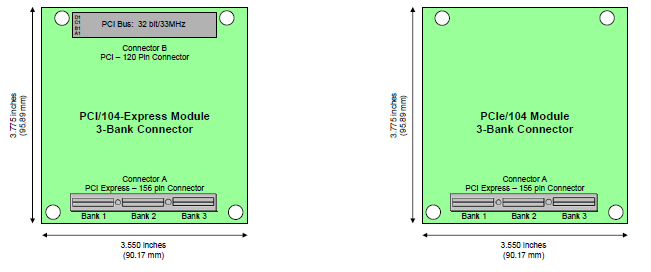
\includegraphics[width=\textwidth]{Img/pci104threebank}
    \caption{Board Layouts de PCI/104-Express y PCIe/104}
    \label{fig:pci104threebank}
\end{figure}

Las estructuras de buses definidos son los que dan lugar a las familias de estándares conocidos del mismo, siendo:

\begin{itemize}
    \item \textbf{PC/104:} Este bus original deriva del bus ISA. Incluye todas las señales encontradas en el mismo, con pines de tierra adicionales agregados para garantizar la integridad del bus.
    \item \textbf{PC/104-Plus:} El mismo agrega soporte para el bus PCI, además del bus ISA del estándar PC/104.
    \item \textbf{PCI-104:} Incluye el conector PCI, pero no el conector PC/104, para aumentar el espacio disponible de la placa. A pesar de que el conector PCI tiene 120 pines en lugar de 104, se mantuvo el nombre establecido. La ubicación del conector PCI y el pinout son idénticos a PC/104-Plus. Dado que se omite el bus ISA, una placa PCI-104 es incompatible con el módulo periférico PC/104. Sin embargo, PCI-104 y PC/104-Plus son compatibles, ya que ambos utilizan el bus PCI. La mayoría de las placas PC/104-Plus pueden fabricarse como PCI-104 simplemente no rellenando el conector PC/104. PCI-104 utiliza el mismo esquema de selección de Número de Ranura PCI que PC/104-Plus. Cada dispositivo debe asignarse a un número de ranura único.
    \item \textbf{PCI/104-Express:} Incorpora el bus PCI Express (PCIe) además del bus PCI de la generación anterior. La especificación define un conector de montaje en superficie de 156 pines para las señales PCI Express. El nuevo conector ocupa la misma ubicación de la placa que el conector ISA PC/104 heredado. Además de PCI Express, las especificaciones también definen los pines en el conector para buses modernos adicionales, como USB y SATA.
    \item \textbf{PCIe/104:} Similar al estándar PCI/104-Express, pero omite el bus PCI heredado para aumentar el espacio disponible en la placa (similar a la relación entre PC/104-Plus y PCI-104). La ubicación del conector PCI Express y las opciones de asignación de patillas son las mismas que para PCI/104-Express (Tipo 1 y Tipo 2). Debido a que se omite el conector de bus PCI, una placa PCIe/104 es incompatible con los sistemas PC/104-Plus y PCI-104 (a menos que se use un dispositivo de puente PCIe a PCI).
\end{itemize}

El factor de forma 104 define el tamaño de la placa (90 * 96 mm), con orificios de montaje en las cuatro esquinas de la placa. Las especificaciones también permiten un área de 0.5 pulgadas (13 mm) más allá del borde de la PCB para los conectores de entrada y salida. La especificación PCI/104-Express y PCIe/104 introdujo el nombre ''104'' para distinguir el factor de forma del bus PC/104 heredado. A su vez, dichas especificaciones aceptan las opciones de uno (Fig. \ref{fig:pci104threebank}) o tres (Fig. \ref{fig:pci104onebank}) \textit{bancos}, agregando mayor flexibilidad al diseñador \cite{pci104express}.

\begin{figure}[!ht]
    \centering
    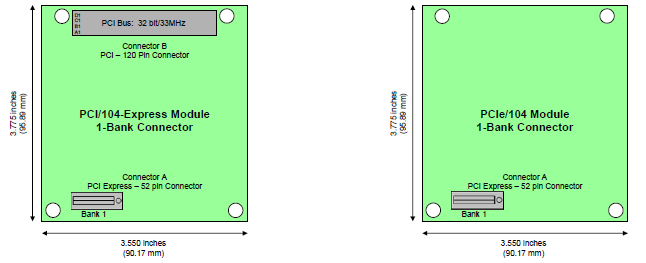
\includegraphics[width=\textwidth]{Img/pci104onebank}
    \caption{Board Layouts de PCI/104-Express y PCIe/104 con conector OneBank}
    \label{fig:pci104onebank}
\end{figure}
    


\newpage
\section{Desarrollo de la solución a implementar}
\label{sec:3_solucion}




\newpage
\section{Resultados, Mediciones y Verificación}
\label{sec:4_resmedver}

\newpage
\section{Conclusiones}
\label{sec:5_concl}

\newpage
\section{Referencias}
\label{sec:6_refs}

\newpage
\section{Bibliografía}
\label{sec:7_biblio}

\begin{thebibliography}{9}
\bibitem{engel2012}
    J. Engel, J. Sturm, and D. Cremers,
    \textit{''Camera-based navigation of a low-cost quadrocopter''}.
    Conference on Intelligent Robots and Systems (IROS),
    2012.
    
\bibitem{engel2014}
    J. Engel, J. Sturm, and D. Cremers,
    ''\textit{Scale-aware navigation of a low-cost quadrocopter with a monocular camera''}.
    Robotics and Autonomous Systems, 
    2014.

\bibitem{hausman2016}
    K. Hausman, S. Weiss, R. Brockers, L. Matthies, and G.S. Sukhatme,
    \textit{''Self-calibrating multi-sensor fusion with probabilistic measurement validation for seamless sensor switching on a UAV''}.
    IEEE International Conference on Robotics and Automation (ICRA),
    2016.

\bibitem{qi2009}
    J. Qi, D. Song, L. Dai and J. Han,
    ''\textit{Design, Implement and Testing of a Rotorcraft UAV System''}.
    Aerial Vehicles, 
    January 2009.

\bibitem{delrosario2016}
    Del Rosario M, Lovell N, Redmond S,
    \textit{''Quaternion-based Complementary Filter for Attitude Determination of a Smartphone''}.
    IEEE Sensors Journal,
    Jun 2016.

\bibitem{caron2006}
    Caron F, Duflos E, Pomorski D, Vanheeghe P,
    \textit{''GPS/IMU data fusion using multisensor Kalman filtering: introduction of contextual aspects''}.
    Information Fusion,
    2006 Jun 30,
    7(2):221-30.
    
\bibitem{mirzaei2008}
    Mirzaei FM, Roumeliotis S,
    \textit{''A Kalman filter-based algorithm for IMU-camera calibration: Observability analysis and performance evaluation''}.
    Robotics, IEEE Transactions,
    2008 Oct,
    24(5):1143-56.

\bibitem{hesch2009}
    Hesch J, Mirzaei FM, Mariottini GL, Roumeliotis S,
    \textit{''A 3d pose estimator for the visually impaired''}.
    IEEE/RSJ International Conference,
    2009 Oct 10,
    (pp. 2716-2723),
    IEEE.
    
\bibitem{chambers2014}
    Chambers A, Scherer S, Yoder L, Jain S, Nuske S, Singh S,
    \textit{''Robust multi-sensor fusion for micro aerial vehicle navigation in GPS-degraded/denied environments''}.
    InAmerican Control Conference (ACC),
    2014 Jun 4, 
    pp. 1892-1899, IEEE.

\bibitem{hesch2013}
    Hesch JA, Kottas DG, Bowman SL, Roumeliotis SI,
    \textit{''Camera-IMU-based localization: Observability analysis and consistency improvement''}.
    The International Journal of Robotics Research,
    2013.

\bibitem{lee2016}
    S. Lee, D. Har, and D. Kum,
    \textit{''Drone-Assisted Disaster Management: Finding Victims via Infrared Camera and Lidar Sensor Fusion''}.
    3rd Asia-Pacific World Congress on Computer Science and Engineering, 
    2016.

\bibitem{shah2017}
    M. Shah, R. Kapdi,
    \textit{''Object detection using deep neural networks''}.
     International Conference on Intelligent Computing and Control Systems (ICICCS),
     2017.
     
\bibitem{autopilot}
    Aautopilot Project,
    \url{https://autopilot-project.eu/}.
    Última vez accedido el 03-08-2018.

\bibitem{pc104}
    PC/104 Embedded Consortium,
    \textit{''PC/104 Specification''}.
    Version 2.6,
    October 13, 2008.

\bibitem{pci104express}
    PC/104 Consortium,
    \textit{''PCI/104-Express \& PCIe/104 Specification''}.
    Version 3.0,
    February 17, 2015
    
\end{thebibliography}


\newpage
\section{Apéndices}
\label{sec:8_apendix}

\subsection{Circuitos electricos}
\label{sec:9_circ}

\subsection{Hojas de Datos}
\label{sec:10_hd}

\subsection{Programas Fuente}
\label{sec:11_soft}

\subsection{Layout PCB}
\label{sec:12_pcblay}

\end{document}